\documentclass[draft=false
              ,paper=a4
              ,twoside=false
              ,fontsize=11pt
              ,headsepline
              ,BCOR10mm
              ,DIV11
              ]{scrbook}
\usepackage[ngerman,english]{babel}
%% see http://www.tex.ac.uk/cgi-bin/texfaq2html?label=uselmfonts
\usepackage[T1]{fontenc}
\usepackage[utf8]{inputenc}     % Zum verwenden von ä,ü und ö: http://en.wikibooks.org/wiki/LaTeX/Special_Characters
\usepackage{libertine,pifont,microtype,textcomp,setspace,makeidx,listings,natbib,soul,hawstyle}
\usepackage[refpage]{nomencl}
\usepackage[colorlinks=true]{hyperref}
\usepackage{lipsum} %% for sample text
\usepackage[nottoc,notlot,notlof,numbib]{tocbibind}
\usepackage{xspace}

% My Commands
\newcommand{\comment}[1]{}

\newcommand{\ac}[0]{$A_C$\xspace}
\newcommand{\seq}[0]{$P_{seq}$\xspace}
\newcommand{\man}[0]{$P_{man}$\xspace}
\newcommand{\ndpn}[0]{$P_{nest}$\xspace}
\newcommand{\ndpv}[0]{$P_{vect}$\xspace}

\newcommand{\algo}[0]{Histogram Balancing\xspace}

\newcommand{\pav}[1][a]{\c{PA #1}\xspace}
\newcommand{\pan}[1][a]{\c{[:#1:]}\xspace}
\newcommand{\pad}[1][a]{\c{Dist (PA #1)}\xspace}

\newcommand{\type}[1]{\c{#1}}
\newcommand{\W}[0]{\textrm{W}}
\newcommand{\D}[0]{\textrm{D}}
\newcommand{\p}[0]{\paragraph{}\xspace}
\renewcommand{\c}[1]{\mbox{\texttt{\footnotesize{#1}}\xspace}}
\newcommand{\lam}[0]{\textrm{$\lambda$}}

\newcommand{\blt}[1]{\textbf{\c{#1}}\xspace}
\newcommand{\pro}[0]{\blt{+}}
\newcommand{\con}[0]{\blt{-}}
\newcommand{\ind}[0]{\blt{ }}

% Building:
% Gedit -> LaTeX build - Strg + Alt + 1
% $ bibtex thesis
% $ makeindex thesis.nlo -s nomencl.ist -o thesis.nls
% Gedit -> LaTeX build - Strg + Alt + 1

% My Packages
\usepackage{booktabs,url}
\usepackage[normalem]{ulem}
\usepackage{graphicx, amsmath}
\usepackage{epigraph}

%% define some colors
\definecolor{keywordblue}{HTML}{5F49CC}
\colorlet{BackgroundColor}{gray!5}
\colorlet{KeywordColor}{keywordblue}
\colorlet{CommentColor}{black!90}
%% for tables
\colorlet{HeadColor}{gray!60}
\colorlet{Color1}{blue!10}
\colorlet{Color2}{white}
  
%% configure colors
\HAWifprinter{
  \colorlet{BackgroundColor}{gray!20}
  \colorlet{KeywordColor}{black}
  \colorlet{CommentColor}{gray}
  % for tables
  \colorlet{HeadColor}{gray!60}
  \colorlet{Color1}{gray!40}
  \colorlet{Color2}{white}
}{}

\lstset{%
  numbers=left,
  numberstyle=\tiny,
  stepnumber=1,
  numbersep=5pt,
  %basicstyle=\ttfamily\small,
  keywordstyle=\color{KeywordColor}\bfseries,
  identifierstyle=\color{black},
  %commentstyle=\color{CommentColor},
  backgroundcolor=\color{BackgroundColor},
  captionpos=b,
  fontadjust=true,
  % mine:
  % frame=none,
  xleftmargin=1em,
  belowcaptionskip=\bigskipamount,
  captionpos=b,
  escapeinside={*'}{'*},
  language=haskell,
  tabsize=0,
  emphstyle={\bf},
  commentstyle=\it,
  stringstyle=\mdseries\rmfamily,
  showspaces=false,
  columns=flexible,
  showstringspaces=false,
  morecomment=[l]\%,
  basicstyle=\ttfamily\footnotesize,
  % keywordstyle=\color{keywordblue},
  keywords={type,if,then,else,let,in}
}
\lstset{escapeinside={(*@}{@*)}, % used to enter latex code inside listings
        morekeywords={uint32_t, int32_t}
}
\ifpdfoutput{
  \hypersetup{bookmarksopen=false,bookmarksnumbered,linktocpage}
}{}

%% more fancy C++
\DeclareRobustCommand{\cxx}{C\raisebox{0.25ex}{{\scriptsize +\kern-0.25ex +}}}

\clubpenalty=10000
\widowpenalty=10000
\displaywidowpenalty=10000

% unknown hyphenations
\hyphenation{
}

%% recalculate text area
\typearea[current]{last}

\makeindex
\makenomenclature

\begin{document}
% \selectlanguage{ngerman}

%%%%%
%% customize (see readme.pdf for supported values)
\HAWThesisProperties{Author={Chandrakant Swaneet Kumar Sahoo}
                    ,Title={Nested Data Parallelism for Image Processing Algorithms}
                    ,SubTitle={Optimisations in Functional Programming Languages}
                    ,EnglishTitle={Nested Data Parallelism for Image Processing Algorithms}
                    ,ThesisType={Bachelorarbeit}
                    ,SubTitleDelimiter={\, -}
                    ,ExaminationType={Bachelorprüfung}
                    ,DegreeProgramme={Bachelor of Science Angewandte Informatik}
                    ,ThesisExperts={Prof. Dr. Michael Köhler-Bußmeier \and Prof. Dr.-Ing. Andreas Meisel}
                    ,ReleaseDate={23. Juli 2015}
                  }

%% title
\frontmatter

%% output title page
\maketitle

\onehalfspacing

%% add abstract pages
%% note: this is one command on multiple lines
\HAWAbstractPage
%% German abstract
{Nested Data Parallelism, Haskell,
Bewertung, Vectorization, Fusion, Histogrammausgleich,
Funktionale Programmierung, Parallele Programmierung, Bildverarbeitung}%
{
Nested Data Parallelism
ermöglicht den prägnanten und treffenden
Ausdruck irregulär-paralleler Programme
und erreicht trotzdessen eine Performance
vergleichbar zu Flat Data Parallelism.
Dies wird durch eine Programmtransformation ('Vectorization')
erreicht. Verschachtelte Funktionen und Datenstrukturen
werden dabei auf flache Funktionen und Datenstrukturen reduziert.
Diese Arbeit verlgeicht und bewertet die Effektivität
von Nested Data Parallelism und manueller Parallelisierung.
Es werden vier Implementierungen des Histogramausgleichs erstellt - 
eine Sequentielle, eine Manuell-parallelisierte,
Eine die NDP verwendet und die davon Vektorisierte.
Diese werden bezüglich Arbeitsaufwand, Ähnlichkeit
zum Algorithmus, Komplexitätklassen und mehr bewertet.
Dies gechieht in Haskell als Example für funktionale Programmiersprachen.
Die Arbeit zieht den Schluss, dass Nested Data Parallelism
effektiv im allgemeinen Verlgeich ist.
Jede Implementierung hat Stärken und Schwächen. Es gibt
allerdings, keine beste Implementierung.}%
%% English abstract
{Nested Data Parallelism, Haskell, Evaluation,
Vectorization, Fusion, Histogram Balancing,
Functional Programming, Parallel Programming,
Image Processing}%
{
Nested Data Parallelism enables
the concise expression of irregularly parallel programs
while still being nearly as performing as flat data parallel programs.
This is achived by a program transformation ('Vectorizaiton')
. It flattens complex nesting of data structures and functions.
This thesis is a comparison and evaluation of nested data parallel
and manually parallelized implementation
of irregular image processing algorithms such as \aglo
in functional programming languages by the example of Haskell.
Four implementations for \algo are created and evaluated on
constant factors, running time complexity, human workload and more. 
They are: sequential, manually-parallelized,
nested data parallel and finally a vectorized thereof.
The thesis comes to the conclusion, that Nested Data Parallelism
compares well to the other approaches.
Though, every implementation has its advantages and drawbacks -
none is the best.}

\newpage
\singlespacing

\tableofcontents
\newpage
%% enable if these lists should be shown on their own page
\listoftables
\listoffigures
%\lstlistoflistings

%% main
\mainmatter
\onehalfspacing
%% write to the log/stdout
%\typeout{===== File: chapter1}
%% include chapter file (chapter1.tex)

\chapter{Introduction}
  
  
  ...
  
  \section{Context}
    ...
  \section{Goal}
    ...
  \section{Structure}
    ...


\chapter{Basics}
  \label{chapter:basics}
  
% Zitat: Auf den Schultern von Riesen.

This chapter will give an introduction into the basics needed to
understand this thesis. We will be introduced into functional programming
in Haskell to ease the understanding of the presented code.
Then we will cover Nested Data Parallelism (NDP) where
key insights are made and concepts exploit them will be presented.
Afterwards a short introduction into parallel complexity measures is given.
We will learn about work and depth complexities, how they relate
to the runtime duraiton and how they can be calculated.
Finally, \algo itself is presented - along with
a description on how it works.

\section{Haskell}
  Haskell is a general purpose, strongly-typed, purely-functional programming
  language. It has full type-inference, referential transparency, higher-order-functions
  and many more features. Traditionally Haskell programming goes by the lines of
  "write what you mean" and "let the compiler do the work for you".
  The former means the use of high abstractions to write concise code -
  while the latter means the use of sophisticated compilers
  \footnote{some which - like the Glasgow Haskell Compiler -  are written in Haskell themselves!}
  to optimise the abstractions to efficient mashine code.
  
  We will now be briefly presented with the main features used in this thesis:
  \paragraph{Syntax}
  Consider this function:
  \begin{lstlisting}
foo :: Double -> Int
foo x = round (max 5 x)
  \end{lstlisting}
  \c{foo} takes the maximum of 5 and the argument number \c{x} and
  rounds it to the nearest integer. The function is given a type
  signature in the first line. \c{f :: t} denotes that \c{f} is of type \c{t}.
  The type describes a function from a double floating number
  to an integer. Multiple argument functions are typed with multiple arrows.
  E.g. \c{max :: Double -> Double -> Double}-
  In contrast to other programming languages parentheses \c{()} are not used for function application
  (as in \c{f(a)}) but instead are used to specify precedence/ordering.
  Function application is done with the most space efficient operator
  one can imagine - that is space ' ' itself! E.g. \c{round 5.2} applies the built-in
  float-rounding function to return the integer \c{5}. Multiple-argument
  functions can be applied with multiple spaces. E.g. \c{max 5 x}
  returns the maximum of 5 and x.
  
  
  We can write the function alternatively as:
  \begin{lstlisting}
foo :: Double -> Int
foo x = let a = max 5 x
                  b = round a
            in  b
  \end{lstlisting}
  \c{let} statements bind expressions to variables.
  The expression after the \c{in} keyword is the return value of the
  entire expression.
  
  
  The upper function can also be written without the explicit use of \c{x}.
  \begin{lstlisting}
foo = (round) . (max 5)
    = round . max 5   -- space has higher precedence than infix operators like .
  \end{lstlisting}
  This is called currying and function composition.
  We can ommit the last argument of a function and define the function
  \c{foo} by literally writing out what we mean:
  "Take the maximum of 5 and then round".
  Function composition is denoted by a dot \c{(.)}.
  
  In Haskell one often ends up nesting multiple functions:
  \begin{lstlisting}
myFunc x = (bar a b (baz c (foo d x)))
  \end{lstlisting}
  We can write the same function in various different ways - depending on space
  and visual ease.
  \begin{lstlisting}
myFunc x = bar a b . baz c . foo d $ x  -- composed with explicit argument
myFunc = bar a b . baz c . foo d        -- composed with implicit argument
myFunc x = bar a b                      -- indented, explicit argument
               . baz c 
               . foo d
               $ x
myFunc = bar a b                        -- indented, implicit argument
             . baz c
             . foo d
  \end{lstlisting}
    The new \c{\$} operator is used here. It - just like the space operator
    - also denotes function application
    \footnote{Fun fact: \c{\$} is defined in Haskell itself! It goes by \c{f \$ x = f x}}
    . However, it
    has very low precedence - so that the functions are composed first
    before the argument is applied into the pipeline of functions.
    Be reminded, that the multi-line definitions actually apply
    the functions from bottom to up. That means, first foo, then baz
    and finally bar is applied - even though foo is written last.
    
  \paragraph{Naming Conventions}
    Higher order functions are denoted with \c{f},\c{g} or \c{h}.
    Usual variables are denoted with \c{x},\c{y},\c{z},\c{a},\c{b},\c{c}
    or with longer names like \c{divisor} or \c{multWith2}.
    If two variables are closly related, then we
    can also write them as \c{x} and \c{x'}. The prime is also
    a part of the variable name.
    Finally, a collection of \c{x} will be refered to by \c{xs}.
    E.g. \c{xs} is an array, \c{xss} is a two dimensional array, and so on.
  
  \paragraph{Strong typing and Type Inference}
    Every expression in has a type. But the programmer doesn't need to
    specify them as they can be (almost always) inferred from the context.
  \paragraph{Type Synonyms}
    Type synonyms enable us to refer to a complicated type by a simpler name.
    E.g. \c{type Foo a = (Int,a)} defines a type synonym - such that
    \c{Foo Double} is replaced by \c{(Int,Double)} during compilation. Compare them to
    type macros.
  
  \paragraph{Referential Transparency and Immutability}
    Functions and expressions are referentially transparent in Haskell 
    (as opposed to 'procedure' or 'object').
    Functions and expressions - like their inspiring equivalent in
    Mathematics - always return the same result when evaluated.
    A consequece is Immutability - variables and data structures
    cannot be mutated. Each function always returns a new copy
    of the data structure. This enables inlining and rewrite rules
    as explored in section \ref{ndpintro}.
    
  \paragraph{Record Syntax}
    We can define records to combine multiple values into a single complex value.
    The following defines a record of type \c{Person} with the
    fields \c{name} and \c{age}
    \begin{lstlisting}
Person {
  name = "Mark"
  age = 23
}
    \end{lstlisting}
    
  \paragraph{Polymorphism}
    Types can be polymorphic. E.g. we can write the general function
    \begin{lstlisting}
foo :: a -> b -> a
foo x y = x
    \end{lstlisting}
    which takes two arguments and simply returns the former only.
    Lower case letters in the type signature denote type variables
    This function works for any arguments - regardless of their types -
    as long as the return type is same as the type of \c{x}. This
    restriction is reflected in the type signature - the first and
    the last type variable have to be equal.
    
    Similarly, we can define functions over polymorphic data types.
    E.g. \c{List a} denotes a list of elements of type a. \c{List Int}
    is for example a linked list of integers.
  
  \paragraph{Higher Order Functions}
    We can define functions which take and pass entire functions as arguments.
    E.g.\c{applyTwice} applies the function twice.
    \begin{lstlisting}
applyTwice :: (a -> a) -> a -> a
applyTwice f x = f (f x)
    \end{lstlisting}
    Note the extra parentheses in the type signature. The type signature
    states "Give me a function from a type \c{a} to itself and an
    argument of type \c{a} then I can return you a value of the same type."
    
  \paragraph{Lambdas}
    We can write literal functions by using lambda expressions.
    For example, the function \c{f x = 2*(x+1)} can also be written
    directly as \c{f = \lam x -> 2*(x+1)} or \c{f = \textbackslash{} x -> 2*(x+1)}.
    The backslash \textbackslash{} is used, when a lambda cannot be written out.
    \footnote{If you bend \textbackslash{} strong enough, you can see its similarity to \lam.}
    
  \paragraph{Identity, flip and function composition (.)}
    Three commonly used functions are:
    
    \begin{lstlisting}
id :: a -> a
id x = x
flip :: (a -> b -> c) -> b -> a -> c
flip f x y = f y x
(.) :: (b -> c) -> (a-> b) -> a -> c
g . f = \x -> g (f x)
    \end{lstlisting}
    where \c{id} is the identity function and \c{flip} exchanges a functions
    first two arguments.
    The identity function is the neutral element of function composition \c{(.)}.
    That menas that (among others) the following law holds:
     \c{\textrm{$\forall$} f: f . id = id . f = f}. This is going to be useful later.

  After a brief overview of the features and a helping hand on the syntax
  I will be using, we can take a look at Nested Data Parallelism.

\section{Nested Data Parallelism}
  \label{ndpintro}
  In the ground breaking work \cite{Belloch1996}
  major contributions to parallel programming in
  functional programming languages were made.
  The paper presented some of Belloch's earlier work (\cite{NepaBelloch1993}) on NESL
  - a programming language specifically designed for expressing parallelism
  in functional programming languages. Its ideas and insights were
  adapted to various languguages - one of them being Haskell.
  Multitude years of research was nesessary to generalize the
  advantages of the special purpose language NESL to a widely used
  general purpose language like Haskell.
  \footnote{For example \cite{Harness2008}, \cite{DPHStatus2007},
  \cite{EffiVect2012Lipp}, \cite{HighOrdFlat2006} and \cite{DistTypes1999}.}
  This project is called Nested Data Parallel Haskell and this section will give
  an overview of its key concepts.  
  
  \paragraph{}
    In Flat Data Parallelism, we are provided with parallel mapping primitives
    to express parallelism. For example, we might have a built-in
    function \c{map} such that \c{map f xs} applies \c{f}
    on each of the elements in the array \c{xs} in parallel.
    
    This function has a farily intuitive parallel implementation -
    simply distribute the input array evenly across the \underline{p}rocessing \underline{u}nits (PUs),
    compute each local chunk of the array with its PU and finally
    join all elements together.
    The inner function \c{f} is applied by each processing unit (PU) individually.
    It is therefore executed sequentially.
    
    This is no problem, if we have statements like \c{map incr}
    \footnote{where \c{incr} increments an integer.}
    . However, what shall we do if we have an expression like \c{map (map incr)}?
    Or even \c{map (map (map incr))}?
    We can only execute the outermost level in parallel because we have already
    distributed the workload among the PUs.
    That means, that the inner function \c{f} can only be executed squentially.
    
    
    This is where NDP can shine. In NDP, in contrast, \c{f} itself can
    also be a parallel operation - and all levels of nesting can
    be executed in parallel! Hence the name - \textbf{Nested} Data Parallelism.
    It does that by transforming the program we wrote into a functionally
    equivalent flat data parallel program. This (non-trivial) transformation
    is called 'flattening' or 'vectoriation' and includes subsequent compiler optimisations.
    All in all, the entire program transformation can be broken down in three steps.
    Each step introduces its new data types.
    \begin{enumerate}
      \item \emph{Vectorization} -
        Uses flat type-dependent array \pav{} representations instead of the
        vanilla nested parallel arrays \pan{} which are used by the programer.
        The flattening is also applied to nested parallel functions as
        those mentioned previously.
      \item \emph{Communicaiton Fusioning} -
        By inlining the definitions of the parallel functions and
        using semantics-preserving rewrite rules one can
        reduce unsessesary synchronisation points and
        create tight pipelines. It uses \pad{} to denote
        distributed chunks of a global array \pav{}.
      \item \emph{Stream Fusioning} -
        Sequential functions local to each PU can further
        be optimised similarly to the previous step
        to reduce the number of intermediate arrays and
        to create tight loops.
        It uses \type{Vector a} and \c{Stream a} to
        implement the local array chunks and to fuse loops, respectively.
    \end{enumerate}
    
  After a overview of the predefined functions - these steps
  are going to be explained in more detail.
  
  \paragraph{}
    For parallel arrays, we have a few predefined operations available.
    They correspond to functions used in conventional functional programming.
    Their names and their types are given in \ref{table:parfuns}.
    
    \begin{table}[h]
      \caption{Parallel functions in NDP}
      \label{table:parfuns}
      \begin{tabular}{lll}
          \toprule
          function & type & description \\
          \midrule
          (!:),indexP & \c{[:a:] -> Int -> a} & indexes the array \\
          lengthP & \c{[:a:] -> Int} & returns the length of the array \\
          headP & \c{[:a:] -> a} & returns the first element\\
          lastP & \c{[:a:] -> a} & returns the last element \\
          mapP & \c{(a -> b) -> [:a:] -> [:b:]} & applies a function on all elements \\
          zipWithP & \c{(a -> b -> c)} & zip together pairs of elements with a \\
           & \c{-> [:a:] -> [:b:] -> [:c:]} & function and return an array of results
           \footnote{e.g. \c{zipWithP (*) [:1,2,3:] [:1,3,4:] = [:1*1,2*3,3*4:]}. The arrays as assumed to be of equal size.}
           \\
          sortP & \c{[:Int:] -> [:Int:]} & sorts an array \\
          sumP & \c{[:Int:] -> Int} & summes the arrays elements \\
          concatP & \c{[:[:a:]:] -> [:a:]} & removes a level of nesting \\
          unconcatP & \c{[:[:a::]] -> [:b:] -> [:[:b:]:]} & exposes a structure to a flat array \\
          replP & \c{Int -> a -> [:a:]} & replicates an element \\
      \end{tabular}
    \end{table}
    
  \subsection{Vectorization}
    Vectorization roughly involves two major steps -
    \emph{Type dependent representation} and \emph{Lifting}.
    Both will be explained in detail now.
  
    \subsubsection{Type dependent representation}
      Type dependent representation 
      allows the programer to work with arrays containing complex
      data structures without sacrifying efficiency.
      
      Consider for example \type{[:Int:]} and \type{[:[:Int:]:]}.
      The former can be easily implemented using a contiguos region
      of memory and inserting the bytes. The latter however cannot
      be implemented equally. What if the sub-arrays are of unequal length?
      To allocate a block of memory, we need to know the size
      of all arrays beforehand.
      Implementing nested array naively would use an array of pointers to
      to arrays of integers. Pointers however are bad, since they
      decrease cache locality and therefore decrease overall performance.
      How can we implement a nested array without using many pointers?
      
      The solution is separation of data and structure.
      The folowing example describes how a nested array
      like \c{[[1,2,3],[4,5],[],[6]] :: [:[:Int:]:]} would be implemented:
      \footnote{\c{[\string#1,2,3\string#]} is the notation used for a contiguos-memory array.}
      \begin{lstlisting}
array :: PA (PA Int)
array = AArr {
  data = [# 1,2,3,4,5,6 #],
  indices = [# 0,3,5,5 #]
  lengths = [# 3,2,0,1 #]
}
      \end{lstlisting}
      All data is packed together into a data field - regardless of nesting -
      and all structucal information is divied into two byte-arrays.
      The indices array contains - for every subarray in the 
      original array - the index of the first element if it were
      to be indexed into the \c{data} field. The lengths describe the lengths of
      each subarray. Each subarray corresponds to a pair of index and length.
      For example, the \underline{second} subarray (\c{[4,5]}) corresponds to
      the \underline{second} index (3) and \underline{second} length (2). Extracting
      2 elements starting at index 3 in the \c{data} array will return
      exactly these two elements.
      Another thing to note; this flat representation
      also uses the new type \type{PA (PA Int)}
      instead of the old \type{[:[:Int:]:]}. 
      Astoundingly, for nested arrays the functions \c{concatP} and \c{unconcatP}
      become constant time operations!
      Removing a level of nesting simply means discarding the segment descriptors -
      and adding a nesting structure of an existing array to a flat array
      means simply adding the segment descriptor of the nested array to the
      flat array.
      
      These crucial insights - namely the flat representation
      of irregularly nested arrays and the constant time
      (un-)flattening operations will be very important later.
      
      
      There are implementation for all other types - such as arrays of ints,
      arrays of doubles, etc. For example \c{[:1,2,3:] :: [:Int:]} can be simply
      represented as:
      \begin{lstlisting}
array :: PA Int
array = AInt [# 1,2,3 #]
      \end{lstlisting}
      
      To finish the data flattening, compiler also transforms
      all normal parallel functions (like \c{fooP}) to
      their predefined scalar counterparts (like \c{fooPS}).
      The scalar functions work directly on the flat representation
      and are designed to exploit them for efficieny.
      This is exactly what \c{concatPS} and \c{unconcatPS} do.
      In fact, functions like \c{fooP} have no actual implementation
      because they are entirely replaced by their \c{fooPS} counterparts.
      They are only used to simpilfy the programmer view.
    
    \nomenclature{Cache Locality}{TODO}
      
    \subsubsection{Lifting}
      During lifting where all occurrences of \c{mapPS f} are
      replaced by \c{fL} and where \c{fL}
      is the lifted version of the original function.
      Compared to the original scalar function \c{f :: a -> b}, the lifted
      function applies the mapping over arrays - alas \c{fL :: PA a -> PA b}.
      For user-defined functions, this lifted function is defined
      by lifting the definition of \c{f} recursively.
      The key is now the definition of the lifted functions for the built-in functions.
      The most important one among them is lifted \c{mapPS} - namely \c{mapPL}.
      To \c{mapPS} of type \c{(a -> b) -> PA a -> PA b},
      \c{mapPL} is of type \c{(a -> b) -> PA (PA a) -> PA (PA b)}.
      To overcome the limitations of flat data parallelsim,
      its implementation has to map over all elements at once
      (instead of mapping over the outer-nesting level only).
      The following implementation does that.
    \begin{lstlisting}
mapPL :: (a -> b) -> PA (PA a) -> PA (PA b)
mapPL f xss =
  unconcatPS xss
  . fL
  . concatPS
  $ xss
    \end{lstlisting}
    The definition of \c{mapPL} is curcial. It is implemented by flattening the array (line 5), applying a flat data-parallel operation (line 4)
    and finally unflattening the new array into the original structure (line 3).
    \footnote{This implementation is different from the original in one important aspect - 
    namely the handling of presupplied arguments in the function. Our
    implementation only handles functions without presupplied arguments -
    but it much simpler to understand than the original in \cite{Harness2008}.
    In the real version we would have another expression \c{expandPS xss fEnv}.
    Introducing it wouldn't affect the overall situation in this thesis -
    so it was simplified.
    }
    Figure \ref{figure:mapP} shall visually aid the understanding by using
    an example of \c{mapP (mapP incr)}.
    
    \begin{figure}[h!]
        \begin{center}
        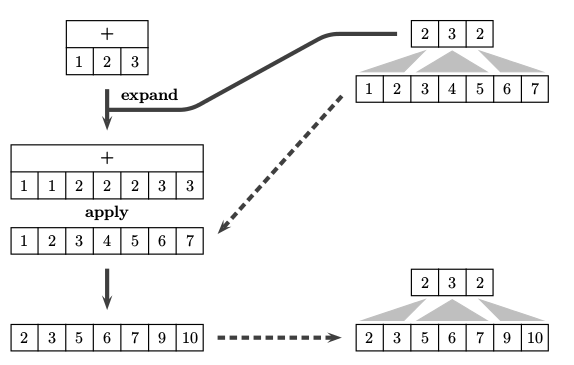
\includegraphics[width=\linewidth]{mapP.png}
        \caption{Conceptional programer view and actual implementation of \c{mapP (mapP incr)}
        \footnote{Here, the commas inbetween the elements have been omitted for visual clarity.
        This thesis will sometimes use such spaces for separation
        instead of commas.
        }
        }
        \label{figure:mapP}
        \end{center}
    \end{figure}
    
    This is the key insight in NDP! Nested Parallel operations - like \c{mapP (mapP incr)} are
    transformed into calls of \c{mapPL incrL} which avoid the nesting of
    the arrays entirely and enable us to map over the entire array in parallel.
    Using this precedure, we can transform nested data parallel programs
    to flat data parallel programs. The former is easy to write and flexible
    - while the latter is simple to implement and efficient in speed.
            
    Vectorization itself is a complex transformation - and many details were ommited.
    More details can be found in \cite{Harness2008}.
    
  \subsection{Communication Fusion}
    During Communication Fusion lifted functions like \c{incrL} are inlined.
    They generally have following form:
    \begin{lstlisting}
incrL :: PA Int -> PA Int
incrL = joinD . mapD incrS . splitD
    \end{lstlisting}
    The types of the new functions are explained in \ref{mapPs}.
    Essentially, the lifted functions are implemented by explicitly
    splitting the array across all PUs, apllying the original
    function (in this case \c{incrS}) on each local chunk sequentially and finally joining all chunks.
    The type \c{Dist a} denotes a distributed value \c{a}.
    Distributable types can be for example arrays or linked lists.
    In case of arrays, the array is chunked and distributed evenly.
    In case of linked lists, the lists can be chunked and
    inter-PU pointers can be used when each chunk reaches its end.
    
    Another aspect to note is the following distinction:
    Using \c{PA a} generally means, that the entire array
    is currently being processed by a single PU and
    then redistributed globally to all PUs.
    Using \c{Dist a} generally means,
    that each PU is currently processing its
    chunk of the distributed value locally.
    
    With such introductions, we can take a look at the type of expressions
    Communication Fusion is designed to optimise. Here is an example.
    \begin{lstlisting}
myFunc :: PA Int -> PA Int
myFunc = mult2L . incrL
    \end{lstlisting}
    where \c{mult2L} is a function which doubles each element in the array.
    Currently, the function works in two steps. First, it splits
    the array, increments and joins the array. Second, it split
    the array, doubles and joins the array again. This is however
    not the optimal approch - and it will be optimised by the compiler.
    
    An effective optimisation strategy in referentially transparent
    programming languages like Haskell are \emph{Inlining}
    \footnote{\cite{Inlining2002}}
    and \emph{Rewrites Rules}
    \footnote{\cite{Simon2001Rewrites}}
    .
    Inlining does what it literally says - it inlines definitions
    of functions and variables. Inlining the definitions
    of the lifted functions reveals the following:
    \begin{lstlisting}
myFunc :: PA Int -> PA Int
myFunc = joinD . mapD mult2S . splitD . joinD . mapD incrS . splitD
    \end{lstlisting}
    Then rewrite rules are used.
    They allow the specification of general semantic-preserving
    laws and allow the compiler to rewrite parts of the code
    according to them.
    They are written by humans and table \ref{rules} introduces a few of them.
    Among them is "splitD/joinD". It states the general law,
    that joining and resplitting an array doesn't change the array at all.
    This is clear for us - but not for the compiler. By specifying such rules
    we can aid the compiler in using equational reasoning to
    optimise the code. In our case the compiler finds the splitD/joinD pair and applies the rule to get:
    \begin{lstlisting}
myFunc :: PA Int -> PA Int
myFunc = joinD . mapD mult2S . mapD incrS . splitD
    \end{lstlisting}
    Applying the rules, the compiler just eliminated
    communication inbetween two phases of computation. This is marvelous!
    Using another rule, namely "mapD/mapD", we can further optimise to.
    \begin{lstlisting}
myFunc :: PA Int -> PA Int
myFunc = joinD . mapD (mult2S . incrS) . splitD
    \end{lstlisting}
    This is even better!
    Communication Fusion did not only reduce the communication but also
    packed together consecutive operations. Now we can further
    optimise local operations using Stream Fusion.
    
    
  \subsection{Stream Fusion}
    Stream Fusion, the optimisation of recursive composed functions
    into a single loop, is a complex topic
    \footnote{A few papers on Stream Fusion:
    \cite{GenVectorFusion2013}, \cite{Fusion2007} and \cite{ArrayFusion2001Chakravarty}
    }
    . We will not go into its details.
    For our purposes it is sufficient to know the following:
    \begin{itemize}
      \item Stream Fusion works very similar to communication fusion
      \item instead of inlining \c{fooL} functions, we inline \c{fooS} functions
      \item instead of mergeing "splitD/joinD" we merge "unstream/stream"
      \item instead of joining "mapD/mapD" we join "mapS/mapS"
      \item \c{Stream a} is a special stream-ful collection with
        non-recursive implementations of various library functions (e.g. \c{mapP},\c{groupP})
        over streams. It is a crucial for the internal optimisation.
      \item Any streams left over after optimisations are converted back into.
        \c{Vector a}. (Since they are the more efficient data container).
    \end{itemize}
    Applying the same procedure creates the following code:
    \begin{lstlisting}
myFunc :: PA Int -> PA Int
myFunc = joinD . mapD (mapS (mult2 . incr)) . splitD
    \end{lstlisting}
    In contrast to our prior - two step - distributed computation,
    our new function has been optimised to communicate only
    at the beginning and the end and to apply both mappings
    in a single loop per PU!
    This is exactly what "let the compiler do the work for you" means!
    
  \subsection{Tables of Functions and Rewrite Rules}
    The transformation in chapter \ref{chapter:ndpv} is going to
    make use of many functions. Most of them are going to be
    introduced when they first appear - others are more frequent
    and require a summary. They are explained in table \ref{mapPs}.
    The table also holds for other functions with same suffix - e.g.
    the \c{mapP} row similarly applies to \c{scanlP}, \c{groupP} etc.
    
    \begin{table}[h!]
      \caption{Overview of Functions and Phases in NDP}
      \label{mapPs}
      \begin{tabular}{lll}
          \toprule
          function & first appearance/ & type/ \\
            & execution context & description \\
          \midrule
          mapP f xs & Programer-view & \type{(a -> b) -> [:a:] -> [:b:]} \\
           & not executed & \textbf{P}arallel array functions the programer uses \\
          mapPS f xs & Vectorization & \type{(a -> b) -> PA a -> PA b} \\
           & not executed & \textbf{P}arallel \textbf{S}calar functions the program is vectorized into \\
          indexPL is xs & Vectorization & \type{PA Int -> PA (PA a) -> PA a} \\
           & not executed & \textbf{P}arallel \textbf{L}ifted indexing on flat arrays. It's scalar\\
           & & function is \type{indexP :: Int -> [:a:] -> a} \\
          mapD f x & Communication Fusion & \type{(Vector a -> Vector b)} \\
           & mapD: all PUs & \type{ -> Dist (PA a) -> Dist (PA b)} \\
           & & Each PU applies \c{f} on it's chunk of the \\
           & f: local per PU & \textbf{d}istributed value. True parallelsim here! \\
          fooS f xs & Communication Fusion & \type{Vector a -> Vector b}\\
           & local PU & Applies a function \textbf{s}equentially. \\
           & & \c{Vector} is the Haskell implementation of \\
           & & conventional PU-local in-memory arrays. \\
          splitD & Communication Fusion & \type{PA -> Dist (PA a)}\\
           & all PUs & splits a glboal array into chunks and \\
           & & distributes them to each of the PUs \\
          joinD & Communication Fusion & \type{Dist (PA a) -> PA a} \\
           & allPUs & join a distributed array into a global array \\
          stream & Stream Fusion & \type{Vector a -> Stream a}\\
           & not executed & convert from an array to a stream-ful data container \\
          unstream & Stream Fusion & \type{Stream a -> Vector a}\\
           & not executed & convert back to an array \\
          mapSt f xs & Stream Fusion & \type{(a -> b) -> Stream a -> Stream b}\\
           & not executed & Applies a function on a \textbf{st}ream of values \\
      \end{tabular}
    \end{table}

    \nomenclature{\c{Vector}}{is the Haskell implementation of conventional local in-memory arrays.
            They are used as the distributed chunks of \pad.}
    
    Most of the functions are simply inlined during optimisation.
    They don't exist anymore at runtime and
    therefore are marked 'not-executed'. Besides these functions, we will also need handful rewrite rules.
    The most important of them are described in table \ref{rules}.
    
    \begin{table}[h!]
      \caption{Rewrite Rules in NDP}
      \label{rules}
      \begin{tabular}{lll}
          \toprule
          rule & rewrite & description \\
          \midrule
          splitD/joinD & splitD . joinD = id & Joining and spliting an distributed array  \\
          & & doesn't change the contents. Therefore \\
          & & it is equivalent to doing nothing. \\
          
          mapD/mapD & mapD g . mapD f & Two consecutive mappings are \\
          & = mapD (g . f) & equivalent to a single mapping \\
          & & with both of the functions \\
          
          mapD/replD & mapD f . replD n & Replicating a value and mapping \\
          & = replD n . f & all values is equivalent to \\
          & & directly applying the function and \\
          & & subsequently replicating it. \\
          
          splitD/replPS & splitD . replPS n & Replicating and spliting a value \\
          & = replD n & is equivalent to creating the local chunks\\
          & & directly. ReplD implements this and knows \\
          & & which chunk its PU is responsible for. \\
          
          ZipReplSplit & zipWithD f (replD a) & Zipping with a replicated value\\
          & . splitD  & already in scope - is equivalent to - applying \\
          & = mapD (f a) & the mapping with the value \\
          & & curried into the function.\\
          
          mapD/zipWithD & mapD f . zipWithD g xs = & A map operation after a zip operation \\
          & zipWithD (\lam x y -> f (g x y)) xs & is equivalent to a single zip operation \\
          & & which applies both \c{f} and \c{g}. \\
          
          unstream/stream & unstream . stream = id & Converting back and fourth is \\
          &  & equivalent to doing nothing. \\
       \end{tabular}
    \end{table}
  
  \subsection{A word on accuracy}
    The project of NDP in Haskell is - even after 15 years -
    still in \textit{work in progress}. Due to frequent changes,
    the papers often use conflicting notation and refer to
    different statuses of progress. Inconsistent literature and a project still in work makes it difficult
    to apply it in a thesis. It is not simple to use the original ideas from
    NESL directly on Haskell as there are great differences (not mentioning
    the fact it already took 15 years to adapt).
    
    Therefore, in this thesis, I have improvised on various conflicting or
    missing details. I assumed implementations which could really have been
    used in NDP.\footnote{E.g. \c{groupP} as introducted in chapter \ref{chapter:ndpn} doesn't
    even exist right now. However, its implementation described there is perfectly possible.}
    The reader is hereby noted that the details
    mentioned here are implementable - but not nesessarily an accurate
    representation of the current state of progress.
    
    
  \paragraph{}
    We have now finally been introduced to the details of NDP and
    are now ready to proceed. The new sections will explain
    parallel complexitiy measures and \algo itself.
  
  \clearpage
  
\section{Parallel Computing and Complexity Measures}
  \label{section:parmeasures}
  In Parallel Computing, the notion of time complexity of implementation
  has to be revisited. Now the time complexity is dependent on the
  number of processors available. Two key measures of
  an algorithm are \emph{work} complexity
  and \emph{depth} complexity. Work is defined
  to be the time (counted in number of operations)
  the algorithms needs, if it were executed on a single processor.
  Depth is defined as the longest chain of sequential data dependency.
  It can also be interpreted as the time needed if we had
  an unlimited number of processors.
  
  There are limited ways in calculating work and depth. Both are defined
  recursively over the work and depths of their subexpressions. Generally,
  work is the sum of operations involved in all of the subexpressions
  - while depths it  the maximum of number of operations involved in
  any particular chain of dependencies.
  We introduce the functions $\W(\cdot)$ and $\D(\cdot)$ which return work
  and depth, respectively. Sometimes we use syntactics constructs
  like $\W(f,x)$ to denote the work involved in \emph{applying}
  \c{f} on \c{x} - it does not include the work involved
  in calculating \c{x} in the first place. Sometimes,
  we will also simple denote $\W(n)$ or $\D(n,gmax)$ to emphasize,
  that the work and depth is dependent of the length of the input
  or of the parameter $gmax$. In these cases. the function refered to
  is clear from the context.
  Table \ref{table:workdepth} gives
  work and depth complexities for our parallel primitives.
  
  \begin{table}[h]
    \caption{Work and Depth complexities of general functions}
    \label{table:workdepth}
    \begin{center}
    \begin{tabular}{lll}
      \toprule
      function & work & depth \\
      \midrule
      (!:),indexP & 1 & 1 \\
      lengthP & 1 & 1 \\
      headP & 1 & 1 \\
      lastP & 1 & 1 \\
      g . f & $\W(g) + \W(f)$ & $\D(g) + \D(f)$ \\
      mapP f xs & 1 + $\W(xs) + \sum_{x \in xs}\W(f,x)$ & 1+ $\D(xs) + \max_{x \in xs}\D(f,x)$ \\
      zipWith f as bs & 1 + $\W(as) + \W(bs)$ & 1 + $\D(as) + \D(bs)$ \\
        & $+ \sum_{pairs (x,y) \in (xs,ys)}\W(f,x,y)$ & $ + \sum_{pairs (x,y) \in (xs,ys)}\D(f,x,y)$ \\
      sortP & $O(n \log n)$ & $O(\log n)$ \\
      sumP & n & $\log$ n \\
      concatP & 1 & 1 \\
      unconcatP & 1 & 1 \\
      replP &  n & 1 \\
    \end{tabular}
    \end{center}
  \end{table}
  
  Note that \c{mapP} has constant depth. 
  It embodies the idea, that the work or depth is the sum or maximum
  of the subexpressions neatly.
  
  Consider for example \c{ys = mapP inrc (replP n 1)}.
  Applying the formulas, we
  get complexities of
  \begin{equation*}
  \begin{split}
  \W(xs)
        & = 1 + \W(replP,n,1) + \sum_{x \in xs}\W(incr,x) \\
        & = 1 + n + n \\
        & \in O(n) \\
  \D(xs) & = 1 + \D(replP,n,1) + \max_{x \in xs}\D(incr,x) \\
      & = 1 + 1 + 1 \\
      & \in O(1) \\
  \end{split}
  \end{equation*}
  where $xs$ is the intermediate array created by \c{replP}.
  Note how we have constant depth!
  If we had as many PUs as our array is in size
  - we could assign each PU one element of the array and our operations
  would indeed require only constant time of local element allocation
  and function application.
  
  These measures, as introduced in \cite{Belloch1996}, work
  neatly within Nested Data Parallelism. Consider for example the
  expression \c{mapP (mapP incr) ass} where the
  nested array \c{ass} has dimensions $w \times h$.
  As we noted in section \ref{ndpintro}, within NDP,
  the nested parallel expression will be flattened into a
  flat array and mapped over only once. Therefore, we expect
  work in $O(w \cdot h)$ and depth in $O(1)$. And indeed - 
  this is what we get when applying our formulas.
  \begin{equation*}
  \begin{split}
  \W(mapP,mapP,incr)
        & = 1 + \sum_{as \in ass}\W(mapP,incr,as) \\
        & = 1 + \sum_{as \in ass}(1 + \sum_{a \in as} \W(incr,a)) \\
        & = 1 + \sum_{as \in ass}(1 + \sum_{a \in as} 1) \\
        & = 1 + \sum_{as \in ass}(1 + h) \\
        & = 1 + w \cdot (1 + h) \\
        & \in O(w \cdot h) \\
  \D(mapP,mapP,incr) & = 1 + \max_{as \in ass}\D(mapP,incr,as) \\
        & = 1 + \max_{as \in ass}(1 + \max_{a \in as} \D(incr,a)) \\
        & = 1 + \max_{as \in ass}(1 + \max_{a \in as} 1) \\
        & = 1 + \max_{as \in ass}2 \\
        & = 1 + 2 \\
        & \in O(1) \\
  \end{split}
  \end{equation*}
  
  Using these constructs, we have a useful tool in measuring
  programs complexity. In the complexities sections of
  the programs, mostly only the results - without their derivaiton -
  will be presented. More detailed derivations of the complexities shown
  in the algorithms sections can be found
  on the appendix.
   
\section{\algo}
  \label{section:hbalanceintro}
  This section will introduce \algo. It will state the problem and give
  an overview of its procedure.
  Suppose we have an $w \times h$-8-bit-gray-tone image with low contrast.
  \footnote{photo by Phillip Capper. Source: \url{https://en.wikipedia.org/wiki/File:Unequalized_Hawkes_Bay_NZ.jpg}}
      
      \begin{figure}[h]
        \centering
        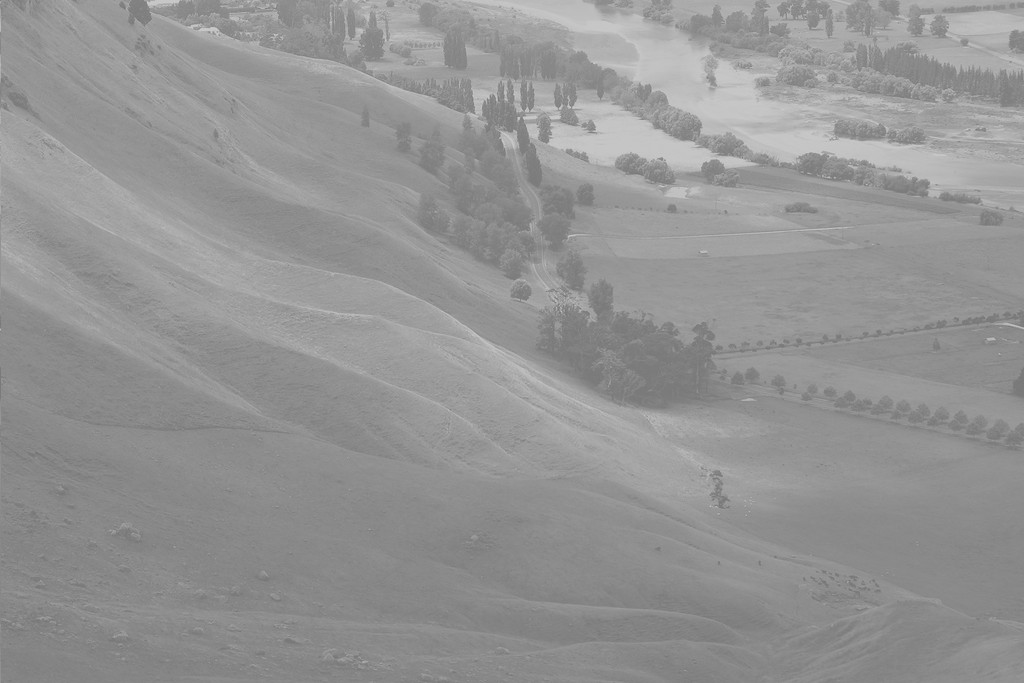
\includegraphics[width=0.45\textwidth]{img-org}
        \caption{An image with low constrast}
        \label{fig:img-org}
      \end{figure}
      Our goal is to make details more visible to the viewer. For that,
      Let's take a look at the histogram of the image.
      \footnote{made by used Wikipedia user \c{Jarekt}. Source: \url{https://en.wikipedia.org/wiki/File:Unequalized_Histogram.svg}}
      
      \begin{figure}[h]
        \centering
        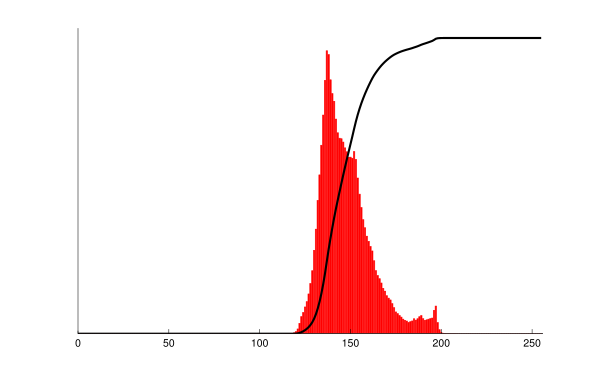
\includegraphics[width=0.45\textwidth]{hist-org}
        \caption{The histogram of the original image with absolute(red) and accumulative(black) count.}
        \label{fig:hist-org}
      \end{figure}
      
      A histogram shows the gray tone distribution of the image in interest.
      The x-axis denotes the gray tone and the y-axis denotes the
      number of pixels with a gray tone $x$ (red). The black curve denotes the
      total number of pixels with a gray tone $g \leq x$.

      We can now see, why details are difficult to recognize in our original image.
      The gray tones are tightly packed together and the
      entire image only uses values in the range [120..205].
      Histogram Balancing solves this problem by defining a mapping
      $f: Graytone \rightarrow Graytone$, such that the accumulating count
      of the resulting image increases as uniformly as possible from 0 to 255.
      The histogram \ref{fig:hist-eq}
      \footnote{made by used Wikipedia user \c{Jarekt}. Source: \url{https://en.wikipedia.org/wiki/File:Equalized_Histogram.svg}}
      shows our goal.
      
      \begin{figure}[h]
        \centering
        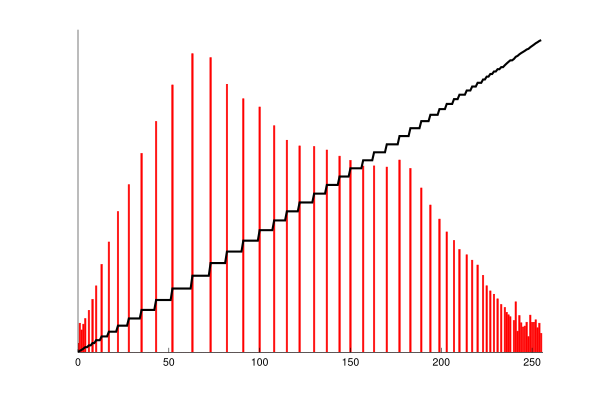
\includegraphics[width=0.45\textwidth]{hist-eq}
        \caption{The histogram of the balanced image}
        \label{fig:hist-eq}
      \end{figure}
      
      Notice the new curve for the accumulating count(black). We can define
      this mapping by spreading out the gray tones such that more
      important gray tones get a larger range to occupy. We interpret
      a high histogram-value for a gray tone as a high importance.
      Given this interpretation, we can - build the accumulation histogram (1 and 2) - remembering which
      bar belongs to which gray tone, normalize(3) and scale(4) the bars to [0..255] - 
      and finally - assign each bar (and therefore its gray tone) a new gray tone
      using the bars location in the range [0..255](5).
      % TODO? I should include visual diagrams for this in the thesis.
      
      \paragraph{}
      To define the transformation $ hbalance: Image \rightarrow Image$ we need the following definitions:
      \begin{itemize}
        \item $Image := (Width,Height,Width \times Height \rightarrow Graytone)$:
          An image
        \item $Histogram_a: Graytone \rightarrow a$:
          A histogram  assigns a value of type $a$ to each gray tone. For $a = Int$,
          this becomes a (accumulated) histogram. For $a = Double$, we get
          a normalised histogram.
        \item $\gmax: Graytone$:
          It is the maximum gray tone for the data type in use. (e.g. 255 for 8-bit gray tones)
      \end{itemize}
      
      Furthermore, the method is broken down into the following functions:
      
      \begin{enumerate}
        \item $hist: Image \rightarrow Histogram_{Int}$
          It calculates the histogram of an image. (1)
        \item $accu: Histogram_{Int} \rightarrow Histogram_{Int}$
          It calculates the accumulating histogram from the original histogram. (2)
        \item $normalize: Int \times Int \times Histogram_{Int} \rightarrow Histogram_{Double}$
          It normalizes the bars (in the range defined by the first two arguments) to a range from 0 to 1. (3)
          The arguments are denoted $a0$ and $agmax$.
          Normalisation is defined by mapping the histogram values by $x \mapsto \frac{(x - a0)}{agmax - a0}$.
          The second argument (called $agmax$) denotes the number of total pixels in the image.
          \comment{
            For an accumulated histogram $a:Histogram_{Int}$ it can be calculated with
            $a(gmax)$ or $a(g')$ where $g'$ is highest gray tone in the image.
            Both are equal, so the implementations may take the liberty to use any of these formulas.
          }
        \item $scale: Graytone \times Histogram_{Double} \rightarrow Histogram_{Int}$
          It scales the normalized values to the maximum gray tone (gmax) and rounds down to the nearest integer.
          Scaling is defined by mapping the histogram values by $x \mapsto \left \lfloor{x \cdot gmax}\right \rfloor $.
        \item $apply: Histogram_{Int} \times Image \rightarrow Image$
          maps each gray tone to its new value as dictated by the first argument. (5)
      \end{enumerate}
      
      Given these functions we can define $hbalance: Image \rightarrow Image$ as:
      \begin{equation*}
      \begin{split}
          h & := hist(img) \\
          a & := accu(h) \\
          s & := scale(gmax,n) \\
          n & := normalize(a(0), a(gmax), a) \\
        hbalance(img) & := apply(s,img) \\
      \end{split}
      \end{equation*}
      
      Concrete implementations will be given in the coming chapters.
      Applying the algorithm to our initial image gives \ref{fig:img-eq}
      \footnote{photo by Phillip Capper. Source: \url{https://en.wikipedia.org/wiki/File:Equalized_Hawkes_Bay_NZ.jpg}}
      . Details are more distinguishable in our new image.
      
      \begin{figure}[h]
        \centering
        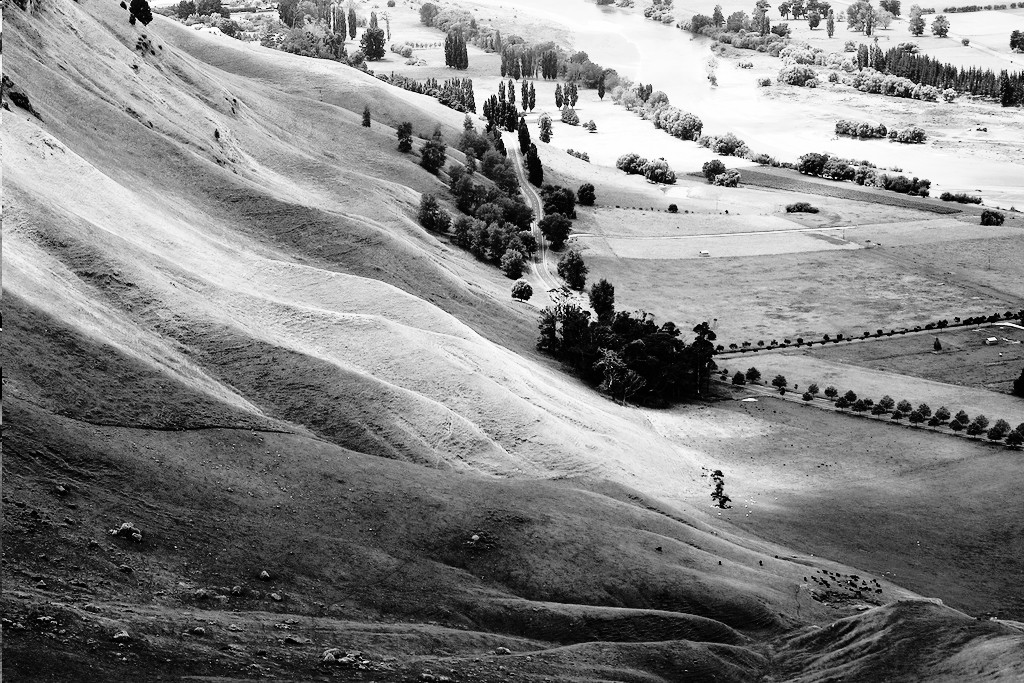
\includegraphics[width=0.45\textwidth]{img-eq}
        \caption{The equalized image}
        \label{fig:img-eq}
      \end{figure}
    
  \algo{} is a frequently used algorithm in image processing. It is 
  one of first methods applied on images to decrease their complexity
  in sophisticated image processing pipelines.
  
  \paragraph{}
  After being exposed to the bread and butter, we are now ready to tackle the
  implementations \seq, \man, \ndpn and \ndpv!
  
  % TODO: cite a book for its uses and the algorithm itself
    
  \comment{
    Prefix sum is a very common operation in computer science. It is a special
      case of scanning through a ordered container from left ro right applying a binary
      associative function \c{f}.
      It is defined as:
        $$ scanl(f,z,[a_1,a_2,...,a_n])
           := [f(z,a_1),f(f(z,a_1),a_2),...,f(f(...f(f(z,a_1),a_2)...,a_{n-1}),a_n)]
        $$
      An example shall be $scanl(+,0,[1,2,2,3,-2]) = [1,3,5,8,6]$. In some definitions
      the first element is $z$. This is however not the definition we need here.
  }

  
\chapter{Sequential: \seq}
  \label{chapter:seq}
  

This chapter introduces \seq - a sequential implementation
of \algo. The implementation is given first. Then
its work and depth complexities - as introduced in section \ref{section:parmeasures}
- are given.


\section{Implementation}
  \seq is a direct implemenation of the description of \algo
  in section \ref{section:hbalanceintro}.
  First the data structures used are presented.
  Then each component of the implementation is given. Afterwards
  the components are assembled to \seq.
  
  \paragraph{Data Structures}
    The implementation uses two data types.
    \begin{lstlisting}
type Image  = PtrVector (PtrVector Int)
type Hist a = TreeMap Int a
    \end{lstlisting}
    \c{PtrVector a} is a pointer-based array holding values
    of type \c{a}. The use of pointers enables them to be nested.
    Thus they can be directly used to represent two-dimensional images.
    \c{TreeMap k a} is a binary search tree indexed by keys of type
    \c{k} and containing values of type \c{a}. They are
    used for the representation of a histogram.
    \footnote{The use of arrays for the representation of
    histograms has undesireable effects. Languges with
    mutability can destructively update the array
    for each pixel in the image. The Immutability
    of Haskell prevents this and forces the use of
    immutable and shared data-structures like \c{TreeMap k a}.}
    
    Functions over \c{PtrVector} are suffixed \c{-V}.
    Functions over \c{TreeMap} aresuffixed \c{-M}.
  
  \paragraph{Histogram Calculation}
    The steps for the creation of the initial histogram are given below:
    \begin{lstlisting}
hist :: Image -> Hist Int
hist = foldrV (\i -> insertWithM (+) i 1) emptyM . concatV
    \end{lstlisting}
    \c{hist} proceeds in two steps. First the image is flatten
    into an one-dimensional array. Then, a \c{TreeMap} is created
    counting the number of occurrences of each gray tone.
    \c{foldrV} is linear in the size of the flattened iamge array.
    \c{insertWithM} is logarithmic in the number elements
    inserted into the map. The size is bounded by the number of 
    gray tones - namely \c{gmax+1}.
    
  \paragraph{Accumulation}
  Calculation the accumulated histogram can be implented by
  a prefix sum over values. It is linear in the size of the map.
  \begin{lstlisting}
accu :: Hist Int -> Hist Int
accu = scanlM (+) 0
  \end{lstlisting}
    
  \paragraph{Normalisation}
  After accumulation, one has to normalise the histogram.
  The normalisation is a direct implementation of its formula in
  \ref{section:hbalanceintro}.
  \begin{lstlisting}
normalize :: Int -> Int -> Hist Int -> Hist Double
normalize a0' agmax' as =
    let a0 = fromIntegral a0'
        agmax = fromIntegral agmax'
        divisor = agmax - a0
    in  mapM (\freq' -> (fromIntegral freq' - a0) / divisor) as
  \end{lstlisting}
  It applies the mapping over the tree-mapusing \c{mapM}.
  \c{fromIntegral} explicitly converts from \c{Int} to \c{Double} since
  Haskell clearly distinguishes them. Variable names with a prime
  (') denote values of type \c{Int}. Variable names without a prime
  denote \c{Double}s. This naming convention is equally used in
  \man, \ndpn and \ndpv.
    
  \paragraph{Scaling}
  Scaling occurs similar to normalisation. It is implemented
  by a mapping over all values in the histogram.
  \begin{lstlisting}
scale :: Int -> Hist Double -> Hist Int
scale gmax = mapM (\d -> floor (d * fromIntegral gmax))
  \end{lstlisting}
    
  \paragraph{Apply}
  The application of the gray tone mapping to the images pixels
  is implemented by a nested \c{mapV} over the image. It uses
  \c{lookupLessEqualM} to lookup the values for the histogram.
  (It reverts back to a lower gray tone, if the gray tone is not found in the map.)
  \begin{lstlisting}
apply :: Hist Int -> Image -> Image
apply as img = mapV (mapV (lookupLessEqualM as)) img
  \end{lstlisting}
  
  \paragraph{\algo}
  Having defined the components, one can now directly define \seq:
  \begin{lstlisting}
hbalance :: Image -> Image
hbalance img =
  let h = hist img
      a = accu h
      a0 = firstM a
      agmax = lastM a
      n = normalize a0 agmax a
      gs = scale gmax n
      img' = apply gs img
  in img'
  \end{lstlisting}
  First the histogram is created (line 3). Then it is accumulated (line 4).
  After that it is normalised (line 5 to 7) and scaled(line 8).
  And finally, the gray tone mapping is applied and returned (line 9 to 10).
  It is defined exactly as previosuly envisioned.
  
\section{Complexities}
  % TODO: continue here.
  USE COST-CENTRE PDF!
  
  Do runtime analysis like in analysis/seq.tex. But a bit less detailed.
  (The actual derivations could be packed into an appendix!)
  
  
  Introduce variables.
  \begin{itemize}
    \item n sei die Anzahl der Bildpixel
    \item w sei die Bildbreite
    \item h sei die Bildhöhe
    \item p sei die Anzahl der PUs (gang members).
  \end{itemize}

  
\chapter{Manually parallelized: \man}
  \label{chapter:man}
  
% Zitat ?

This chapter will give an implementation of \algo
that cannot make use of NDP. This is
the case when one is only given a few parallel primitives
that don't support nesting
of operations (at least not without falling back to sequential evaluation).
Table \ref{table:parprims} shows a few of these primitives.

  \begin{table}[h!]
    \caption{Parallel Primitives in Flat Data Parallelism}
    \label{table:parprims}
    \begin{center}
    \begin{tabular}{lll}
      \toprule
      function & type \\
      \midrule
      parMap & \c{(a -> b) -> Vector a -> Vector b} \\
      parZipWith & \c{(a -> b -> c)} \\
       & \c{Vector a -> Vector b -> Vector c} \\
      parReplicate & \c{Int -> a -> Vector a} \\
      parGenerate & \c{Int -> (Int -> a) -> Vector a} \\
    \end{tabular}
    \end{center}
  \end{table}
  They are analogous to the parallel functions in NDP.
  \c{parGenerate} is a function such that \c{parGenerate size f} creates a new array
  of size \c{size} and uses the generator function \c{f} to create
  the elements by their indices.
  E.g. \c{parGenerate 5 (\lam i -> i*i) = [0,1,4,9,16] }.
  These primitives all have work $O(n)$ and depth $O(1)$.
  
\section{Parallel histogram accumulation}
  To implement \algo in parallel, one has to revisit the sequential
  implementation. The parallel creation of the accumulated histogram is
  a difficult task. The goal is to try to come up with
  an low complexity algorithm for the histogram calcuation.
  After a few tries, one can give the following implementation:
  
  \begin{lstlisting}
accuHist :: Image -> Hist
accuHist []  = parReplicate gmax 0
accuHist [x] = parGenerate gmax (\i -> if (i >= x) then 1 else 0)
accuHist xs  = let (left,right) = splitMid xs
                   [leftRes,rightRes] = parMap accuHist [left,right]
               in  parZipWith (+) leftRes rightRes
  \end{lstlisting}
  The general idea is to merge accumulation and histogram creation
  into a single tree-like reduction. To each array of pixels, \c{accuHist}
  returns the accumulated histogram of its gray tones.
  The algorithim can be broken down into two edge-cases and one recursive case
  . Figure \ref{figure:accuHist} gives an example of its evaluation.
  
  \begin{figure}[h]
    \centering
    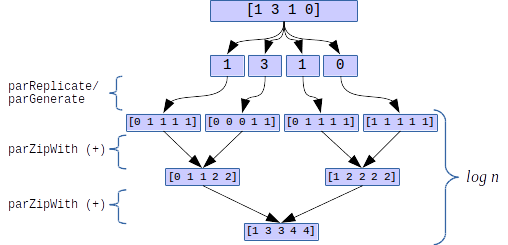
\includegraphics[width=\linewidth]{accuHist}
    \label{figure:accuHist}
    \caption{Evaluation of \c{accuHist [1,3,1,0]}}
  \end{figure}
  
  Suppose \c{gmax = 4} then the algorithm returns \c{[0 0 0 0 0]} if
  the input array was empty. If the image only contained a single gray tone
  \c{x}, then it creates its accumulated histogram
  \c{[0 0 ... 0 1 ... 1 1]} such that \c{x} is the index
  of the first \c{1}.
  For example, for \c{x = 2} the array
  \c{[0 0 1 1 1]} is returned. This is implemented using the \c{parGenerate} function.
  Finally, one has the recursive case. In this case, the the calculation
  of larger images is broken down by splitting the array into half
  \footnote{splitting is a constant time operation
  for these view-based arrays} and applying \c{accuHist}
  recursively. Finally, the histograms are merged with elementwise addition
  ({\c{zipWith(+)}}).
  
  This algorithm was carefully constructed after many failed approaches
  on such an algorithm. Alternatives were considered, but they did not
  yield an acceptable complexity compared to \c{accuHist}.

\section{Implementation}
  Given the introduction, the manurally parallised \man can finally be implemented.
  The parallel primitives can be integrated
  well into normalisation and scaling.
  However, \c{accuHist} and \c{apply} need to be adapted.
  The code is given below. \c{(!)} is used for indexing.
  \begin{lstlisting}
type Image  = Vector Int
type Hist   = Vector Int

hbalance :: Image -> Image
hbalance img =
  let hist = accuHist img
      a0 = hist ! 0
      agmax = hist ! gmax
      apply gs = parMap (\i -> gs ! i) img
      sclNrm :: Int -> Int
      sclNrm x = floor ( (x-a0)/(agmax - a0)*gmax )
  in  apply (parMap sclNrm) hist
  \end{lstlisting}
  As explained in the previous section, the parallel
  accumulated histogram calculation has been implemented in \c{accuHist}.
  For the gray tone mapping (\c{apply}) to work, nested arrays cannot be used
  \footnote{as they would result into an array of pointers to subarrays.
  This is undesireable due to Cache Locality.}
  .
  One needs to change the entire image representation to a flat array manually.
  To retrieve a specific pixel one needs to calculate
  the offset using the image's width. Fortunately,
  for \algo, indexed retrieval of pixels is not needed.
  However, any subsequent algorithms in the pipeline of image processing
  would have to cope with the flat image representation directly.
    
\section{Complexities}
  In this section, complexitiy measures for the functions
  involved in \man will be given.
  To calculate work and depth of \man, one needs the measures of
  all subfunctions and subexpressions. \c{accuHist} is
  not a built-in function - and so needs an individual analysis first.
  
  \paragraph{\c{accuHist}}
    The recursive case of \c{accuHist} involves functions
    of work $O(gmax)$ and depth $O(1)$ - 
    namely \c{parZipWith (+)} and \c{splitMid}.
    The exceptions are the two recursive calls (packed together into a
    \c{parMap}).
    
    One can state the work of \c{accuHist} as a recursive function
    \begin{equation*}
    \W(n,gmax) = \begin{cases}
                 gmax & \text{ if } n \le 1 \\ 
                 2 \W(\frac{n}{2}) + gmax & \text{ else }
                \end{cases} \\
    \end{equation*}
    where the edge-cases and recursive-cases correspond one-to-one
    to the definition of \c{accuHist}.
    Such a recurrence relation can be resolved by tying the knot
    or using the Master Theorem's first case
    \footnote{Master theorem: \cite{Cormen2001}}
    \footnote{However, the Master Theorem doesn't apply directly
    because it treats \c{gmax} as a constant -
    and not as a variable parameter.
    The Master Theorem would give $O(n)$ whereas tying the knot
    would give the more accurate class $O(n \cdot gmax)$.}
    .
    The following equations shall tie the knot:
    \begin{equation*}
    \begin{split}
    \W(n,gmax)
      & = \begin{cases}
            gmax & \text{ if } n \le 1 \\ 
            gmax2^0 + 2^1\W(\frac{n}{2}) & \text{ if } n = 2 \\
            gmax2^0 + gmax2^1 + 2^2\W(\frac{n}{4}) & \text{ if } n = 3 \\
            gmax2^0 + gmax2^1 + ... + gmax 2^{\log n - 1} + 2^{\log n}\W(1) & \text{ else }
          \end{cases} \\
      & = \textrm{ (... tying the knot ...) } \\
      & = gmax \sum_{i=0}^{\log n}{2^i} \\
      & = gmax (2^{\log n + 1} - 1) \\
      & = gmax (2n - 1) \\
      & \in O(n \cdot gmax) \\
    \end{split}
    \end{equation*}
    
    Such a tree-like reduction has height logarithmic
    in the size of the input array. The input array is the image and
    has size \c{n}. Therefore, one can conclude
    $\D(n, gmax) \in O(\log n)$.
  
  \paragraph{Putting it together}
    Given the code for \man, one can now give work and depth
    complexities. These complexities are given in table \ref{table:man}.
    The table summarises the work and depths of each of the calls.
    
  \begin{table}[h]
    \centering
    \caption{Work and Depth complexities}
    \label{table:man}
    \begin{tabular}{lll}
        \toprule
        function or variable & O(W)     & O(D) \\
        \midrule
        hbalance        & n * gmax      & log n \\
        apply           & n           & 1 \\
        parMap sclNrm   & gmax        & 1 \\
        accuHist     & n * gmax      & log n \\
        \midrule
        accuHist     & n * gmax      & log n \\
        splitMid        & 1           & 1 \\
        parZipWith      & gmax        & 1 \\
        parReplicate       & gmax        & 1 \\
        parGenerate        & gmax        & 1 \\
        arr ! i          & 1           & 1 \\
    \end{tabular}
  \end{table}
  
  By applying the formulas, from section
  \ref{section:parmeasures} one can calculate the table.
  The outer-most work and depth of \man is given below:
  \begin{equation*}
  \begin{split}
  \W(n,gmax)
        & = \W(accuHist) + \W(parMap,sclNrm) + \W(apply) \\
        & = n \cdot gmax + gmax + n \\
        & \in O(n \cdot gmax) \\
  \D(n,gmax)
      & = \max \{ accuHist, (parMap,sclNrm), apply\} \\
      & = \max \{ \log n, 1, 1\} \\
      & \in O(\log n) \\
  \end{split}
  \end{equation*}
  
  One can note, how work and depth of \man is entirely bounded
  by the complexities of \c{accuHist}. Improvements to \c{accuHist}
  complexities will improve \man either.
  
  \paragraph{}
  Before moving to the next chapter - one shall be reminded that
  \man involved much manual work. It was not a direct translation
  of the algorithms description. It, especially requires
  the subsequent algorithms to use a flat image representation.
  
  
  The next chapter covers \ndpn - an implementation using NDP.
  
  
  
  


\chapter{Nested-Data-Parallel: \ndpn}
  \label{chapter:ndpn}
  \documentclass{article}

% Latex Tutorial beginners: http://www.latex-tutorial.com/tutorials/beginners/


% Packages explained - Adding more functions to LATEX http://www.latex-tutorial.com/tutorials/beginners/lesson-3/
\usepackage[utf8]{inputenc}     % Zum verwenden von ä,ü und ö: http://en.wikibooks.org/wiki/LaTeX/Special_Characters
\usepackage{booktabs}
\usepackage{url}
\usepackage{hyperref}
\usepackage[T1]{fontenc}
\usepackage[margin=1.3in]{geometry}
\usepackage[nottoc,notlot,notlof,numbib]{tocbibind}
\usepackage{listings,xcolor}
\usepackage{amsmath}


\newcommand{\comment}[1]{}

\newcommand{\seq}[0]{$P_{seq}$}
\newcommand{\man}[0]{$P_{man}$}
\newcommand{\ndpn}[0]{$P_{nest}$}
\newcommand{\ndpv}[0]{$P_{vect}$}
\newcommand{\algo}[0]{Histogram Balancing}
\newcommand{\type}[1]{\texttt{#1}}
\newcommand{\ts}[0]{\,}% type space
\newcommand{\Hist}[1]{[:\ts#1\ts:]}
\newcommand{\pa}[1]{[:#1:]}

\newcommand{\eqdo}[0]{\hskip 4em}
\newcommand{\W}[0]{\textrm{W}}
\newcommand{\D}[0]{\textrm{D}}

\definecolor{keywordblue}{HTML}{5F49CC}
\lstset{
  frame=none,
  xleftmargin=2pt,
  belowcaptionskip=\bigskipamount,
  captionpos=b,
  escapeinside={*'}{'*},
  language=haskell,
  tabsize=2,
  gobble=6,
  emphstyle={\bf},
  commentstyle=\it,
  stringstyle=\mdseries\rmfamily,
  showspaces=false,
  columns=flexible,
  showstringspaces=false,
  morecomment=[l]\%,
  basicstyle=\ttfamily,
  keywordstyle=\color{keywordblue},
  keywords={type,if,then,else,let,in}
}

\begin{document}

    \section{ \ndpn }
      \begin{lstlisting}
        type Image = [:[:Int:]:]
        type Hist a = [:a:]

        hbalance :: Image -> Image
        hbalance img =
            let h = hist img
                a = accu h
                a0 = headP a
                agmax = lastP a
                n = normalize a0 agmax a
                s = scale gmax n
                img' = apply s img
            in  img'

        hist :: Image -> Hist Int
        hist = 
            sparseToDenseP (gmax+1) 0
            . mapP (\g -> (headP g,lengthP g))
            . groupP
            . sortP
            . concatP

        accu :: Hist Int -> Hist Int
        accu = scanlP (+) 0

        normalize :: Int -> Int -> Hist Int -> Hist Double
        normalize a0' agmax' as =
            let a0 = fromIntegral a0'
                agmax = fromIntegral agmax'
                divisor = agmax - a0
            in  [: (fromIntegral freq' - a0) / divisor | freq' <- as :]

        scale :: Int -> Hist Double -> Hist Int
        scale gmax as = [: floor (a * fromIntegral gmax) |  a <- as :]

        apply :: Hist Int -> Image -> Image
        apply as img = mapP (mapP (as !:)) img
      \end{lstlisting}
    
    \newpage
    
    \section{Work and Depth Table}
      
      \begin{itemize}
        \item n sei die Anzahl der Bildpixel
        \item w sei die Bildbreite
        \item h sei die Bildhöhe
        \item p sei die Anzahl der PUs (gang members).
      \end{itemize}
      
      \paragraph{}
        \begin{table}[h]
          \caption{Work and Depth complexities}
          \label{timetable}
          \begin{tabular}{lll}
              \toprule
              function or variable &      O(W)           & O(D) \\
              \midrule
              hbalance        & \max(n \log n, gmax) & \log \max(n, gmax) \\
              \midrule
              hist            & \max(n \log n, gmax) & log n \\
              sparseToDenseP  & gmax                 & 1 \\
              groupP          & n                    & \log n \\
              sortP           & n \log n             & \log n \\
              concatP         & 1                    & 1 \\
              \midrule
              accu            & gmax                 & \log gmax \\
              scanlP          & gmax                 & \log gmax \\
              \midrule
              normalize       & gmax                 & 1 \\
              scale           & gmax                 & 1 \\
              \midrule
              apply           & $n = w \cdot h \cdot O(1)$ & 1 \\
              mapP f xs       & $W(f,x) \cdot size(xs)$      & 1 \\
              headP/lastP     & 1                    & 1 \\
              indexP, !:      & 1                    & 1 \\
          \end{tabular}
        \end{table}
      
    \section{Other aspects \small{e.g. sync-points, programmer workload, simplicity}}
      \begin{itemize}
        \item optimisations: no optimisations. Uses many synchronisation points
          (the many bulkd-functions imply much communication)
        \item progammer-workload: failry easy to write. I had written it in less than 1 hour.
        \item simplicity: Implementation can be understood without comments, however needs some time.
      \end{itemize}
      

\end{document}





\chapter{Vectorized Nested-Data-Parallel: \ndpv}
  \label{chapter:ndpv}
  \documentclass{article}

% Latex Tutorial beginners: http://www.latex-tutorial.com/tutorials/beginners/


% Packages explained - Adding more functions to LATEX http://www.latex-tutorial.com/tutorials/beginners/lesson-3/
\usepackage[utf8]{inputenc}     % Zum verwenden von ä,ü und ö: http://en.wikibooks.org/wiki/LaTeX/Special_Characters
\usepackage{booktabs}
\usepackage{url}
\usepackage{hyperref}
\usepackage[T1]{fontenc}
\usepackage[margin=1.3in]{geometry}
\usepackage[nottoc,notlot,notlof,numbib]{tocbibind}
\usepackage{listings,xcolor}
\usepackage{amsmath}


\newcommand{\comment}[1]{}

\newcommand{\seq}[0]{$P_{seq}$}
\newcommand{\man}[0]{$P_{man}$}
\newcommand{\ndpn}[0]{$P_{nest}$}
\newcommand{\ndpv}[0]{$P_{vect}$}
\newcommand{\algo}[0]{Histogram Balancing}
\newcommand{\type}[1]{\texttt{#1}}
\newcommand{\ts}[0]{\,}% type space
\newcommand{\Hist}[1]{[:\ts#1\ts:]}
\newcommand{\pa}[1]{[:#1:]}

\newcommand{\eqdo}[0]{\hskip 4em}
\newcommand{\W}[0]{\textrm{W}}
\newcommand{\D}[0]{\textrm{D}}

\definecolor{keywordblue}{HTML}{5F49CC}
\lstset{
  frame=none,
  xleftmargin=2pt,
  belowcaptionskip=\bigskipamount,
  captionpos=b,
  escapeinside={*'}{'*},
  language=haskell,
  tabsize=2,
  gobble=6,
  emphstyle={\bf},
  commentstyle=\it,
  stringstyle=\mdseries\rmfamily,
  showspaces=false,
  columns=flexible,
  showstringspaces=false,
  morecomment=[l]\%,
  basicstyle=\ttfamily,
  keywordstyle=\color{keywordblue},
  keywords={type,if,then,else,let,in}
}

\begin{document}

    \section{\ndpv}
      \begin{lstlisting}
        type Image = PA (PA Int)
        type Hist  = PA Int

        hbalance :: Image -> Image
        hbalance img =
          let a :: Hist                                     -- Histogram
              a = joinD                                     -- accu end
                  . mapD (\(as,a) -> mapS (plusInt a) as)
                  . propagateD plusInt 0
                  . mapD (scanlS plusInt 0)                 -- accu begin
                  . sparseToDenseD (plusInt gmax 1) 0       -- hist end
                  . splitSparseD (plusInt gmax 1)
                  . joinD
                  . mapD tripletToATup2
                  . segdSplitMerge 0
                  . sortPS
                  . concatPS                                -- hist begin
                  $ img                                     -- 1
                      
              n :: Int
              n = lengthPS a                                -- 2
              
              a0, divisor, gmax' :: Double
              a0      = int2Double . headPS $ a             -- 3, variables for normalize and scale
              divisor = minusDouble (int2Double (lastPS a)) . int2Double . headPS $ a
              gmax'   = int2Double $ gmax
              
              normScale :: Int -> Int                       -- 0, body of normalize and scale
              normScale =
                floorDouble
                . (flip multDouble) gmax'
                . (flip divDouble) divisor
                . (flip minusDouble) a
                . int2Double
              
              as :: Hist                                    -- final mapping array
              as = joinD . mapD (mapS normScale) . splitD $ a -- 4, normalize and scale applied
              
              pixelReplicate :: Hist -> PA Hist             -- 0, artifact of NDP
              pixelReplicate = concatPS . replPL (lengths (getSegd xs)) . replPS (lengthPS img)
              
          in unconcatPS img
             . indexPL (pixelReplicate as)                  -- 5, apply. core of nested data parallelism here!
             . concatPS
             $ img
      \end{lstlisting}
    
    \newpage
    
    \section{Work and Depth Table}
      
      \begin{itemize}
        \item n sei die Anzahl der Bildpixel
        \item w sei die Bildbreite
        \item h sei die Bildhöhe
        \item p sei die Anzahl der PUs (gang members).
      \end{itemize}
      
      \paragraph{}
        \begin{table}[h]
          \caption{Work and Depth complexities}
          \label{timetable}
          \begin{tabular}{lll}
              \toprule
              function or variable &      O(W)           & O(D) \\
              \midrule
              hbalance        & \max(n \log n, gmax)& \log \max(n, gmax) \\
              \midrule
              hist            & \max(n \log n, gmax)& \log n \\
              concatPS        & 1                   & 1 \\
              sortPS          & $n \log n$          & $\log n$ \\
              segdSplitMerge  & $n \log n$          & $\log n$ \\
              mapD tripletToATup2  & gmax           & 1 \\
              joinD xs        & gmax                & 1 \\
              \midrule
              accu            & gmax                & \log gmax \\
              sparseToDenseD  & gmax                & 1 \\
              splitSparseD    & gmax                & 1 \\
              mapD scanlS     & gmax                & 1 \\
              propagateD      & 1                   & $\log gmax$ \\
              mapD (mapS plusInt) & gmax            & 1 \\
              joinD           & gmax                & 1 \\
              \midrule
              as              & gmax                & 1 \\
              splitD          & gmax                & 1 \\
              mapD normScale  & gmax                & 1 \\
              joinD           & gmax                & 1 \\
              \midrule
              pixelReplicate  & 1 (bzw. $n \cdot gmax$) & 1 \\
              \midrule
              img'            & n                   & 1 \\
              concatPS        & 1                   & 1 \\
              indexPL         & n                   & 1 \\
              unconcatPS      & 1                   & 1 \\
              \midrule
              & general complexities & \\
              mapD fS xs      & $\W(fS,s)*size(xs)$ & $\W(fS,s)*size(xs)/p$ \\
              joinD xs        & size(xs)          & 1 \tiny (communication overhead?) \\
              splitD xs       & size(xs)          & 1 \tiny (communication overhead?) \\
              replPS n x      & n                   & 1 \\
              replPL ns xs    & sum(ns)*size(xs)    & 1 \\
              sortPS xs       & $size(xs) \log size(xs)$ & $\log size(xs)$ \\
          \end{tabular}
        \end{table}
        
    \section{Calculating "hbalance" entirely}
      Let $n = |img| = w\cdot h$
      \begin{equation}
      \begin{split}
      \W(w \times h,gmax)
            & = \W(hist) + \W(accu) + \W(as) + \W(pixelReplicate) + \W(img') \\
            & = O( \max(n \log n, gmax) + gmax + gmax + 1 + n) \\
            & \in O(\max(n \log n, gmax)) \\
      \D(w \times h,gmax)
          & = \max \{ hist, accu, as, pixelReplicate, img'\} \\
          & = \max \{\log n, \log gmax \} \\
          & \in O(\log \max(n,gmax)) \\
      \end{split}
      \end{equation}
        
    \section{Calculating the histogram "hist"}
      Let $n = |img| = w\cdot h$
      \begin{equation}
      \begin{split}
      \W(w \times h)
            & = \W(concatPS) + \W(sortPS) + \W(segdSplitMerge) \\
            & + \W(mapD,tripletToATup2) + \W(joinD) \\
            & = 1 + n \log n + n \log n + gmax + gmax \\
            & = 1 + 2 (n \log n + gmax) \\
            & \in O(\max(n \log n, gmax)) \\
      \D(w \times h)
            & = \max \{ concatPS,sortPS,...,joinD\} \\
            & \in O(\log n) \\
      \end{split}
      \end{equation}
    
    \section{Calculating the accumulated histogram "accu"}
      \begin{equation}
      \begin{split}
      \W(gmax)
            & = \W(splitSparseD) + \W(sparseToDenseD) + \W(mapD,scanlS) \\
            &     + \W(propagateD) + \W(mapD,mapS,plusInt) + \W(joinD) \\
            & = gmax + gmax + gmax + 1 + gmax + gmax\\
            & = 1 + 5 \cdot gmax \\
            & \in O(gmax) \\
      \D(gmax)
          & = \max \{ splitSparseD, sparseToDenseD, (mapD,scanlS),...\} \\
          & \in O(\log gmax)
      \end{split}
      \end{equation}
    
    \section{Calculating the mapping array "as"}
      \begin{equation}
      \begin{split}
      \W(gmax)
            & = \W(joinD) + \W(mapD,normScale) + \W(splitD) \\
            & = gmax + gmax + gmax \\
            & = 3 \cdot gmax \\
            & \in O(gmax) \\
      \D(gmax)
          & = \max \{ joinD,(mapD,normScale),splitD\} \\
          & \in O(1)
      \end{split}
      \end{equation}
      
    \section{Calculating by "pixelReplicate"}
      PixelReplicate is a function which executed strictly
      and literally would have a work complexity of $n \cdot gmax$.
      However, due to strong improvements in [WorkEfficient]
      this replication is simply cached locally such that
      the work complexity for this case is negilible and
      can be simplified to $1$.
      
      \begin{equation}
      \begin{split}
      \W(gmax,w \times h)
            & \in O(1) \\
      \D(gmax, w \times h)
            & \in O(1) \\
      \end{split}
      \end{equation}
      
    \section{Calculating the final balanced image "img'"}
      \begin{equation}
      \begin{split}
      \W(gmax, w \times h)
            & = \W(unconcatPS) + \W(indexPL) + \W(concatPS) \\
            & = 1 + n + 1 \\
            & \in O(n) \\
      \D(gmax, w \times h)
          & = \max \{ unconcatPS, indexPL, concatPS \} \\
          & \in O(1)
      \end{split}
      \end{equation}
      
    \section{Other aspects \small{e.g. sync-points, programmer workload, simplicity}}
      \begin{itemize}
        \item optimisations:
          removed sync-points(more local operations),
          tight distributed normalisation loop,
          distributed optimal prefix-sum,
          distributed groupP and sortP,
          nested data parallelism enables a depth lower than O(width)
        \item progammer-workload: compiler does all the optimisations. as much as for \ndpn
        \item simplicity: hard to comphrehend, not indented for human readers, but shows optimisations clearly
      \end{itemize}
      

\end{document}





\chapter{Results and Discussion}
  \label{chapter:results}
  
% Vertrauen ist gut, Kontrolle ist besser.

This chapter summarises results of the four implementations
\seq, \man, \ndpn and \npdv. First the complexities of
the programs are given and observations
are made an discussed.
Then, the pro and contra of each program are given - 
comparing them on different aspects.
Finally, the chapter ends with a conclusion.

\section{Complexity Analysis}
  The complexities of all four programs are summarised in table
  \ref{table:allcomps}. Note that in most image processing applications $gmax < n$ holds. The number
  of pixels in an image is usually greater than the 
  number of gray tones each pixel has available.
  
  \begin{table}[h!]
    \caption{Work and Depth complexities}
    \label{table:allcomps}
    \centering
    \begin{tabular}{lll}
      \toprule
      program & work & depth \\
      \midrule
      \seq  & $n \log gmax + gmax$ & $n \log gmax + gmax$ \\
      \man  & $n \cdot gmax$ & $\log n$ \\
      \ndpn & $n \log n + gmax$ & $\log n + \log gmax$ \\
      \ndpv & $n \log n + gmax$ & $\log n + \log gmax$ \\
    \end{tabular}
  \end{table}
  A few observations can be made.
  
  \paragraph{\ndpn versus \ndpv:}
    \ndpn and \ndpv have equal work and depth complexities.
    Compiler optimisations can rarely optimise into a lower complexity class.
    However, the use of flat data structures, the optimisation
    for cache locality and the fusion of communication and loops
    greatly reduces the constants factors of \ndpv.
  
  \paragraph{\man versus \ndpv:}
    \label{paragraph:manvsndpv}
    Work and depth complexities of \man and \ndpv are competing.
    While the work of \man is a product of the parameters $n$ and $gmax$ - 
    the work of \ndpv (and \ndpn) is only a sum. For larger parameters,
    and a limited number of processors \ndpv will out-compete \man.
    \ndpv has a speed-up linear in $gmax$.
    
    Regarding depth however, the opposite is the case. \man grows
    logarithmic to $n$ whereas \ndpv grows logarithmic
    to $n$ and $gmax$. For large values of $gmax$ and a high number of processors,
    \man will out-compete \ndpv. However, the speed-up is only a
    summand of $\log gmax$.
  
  \paragraph{Sequential versus Parallel:}
    \seq has the best bounds in work out of all programs.
    It is low due to its iteration-based histogram creation.
    Parallel programs cannot use this method because they
    then were to fall back to sequential traversal.
    \man and \ndpn instead used more advanced methods to implement the histogram creation
    in parallel.
    
    On the one hand, their methods have worse work complexities.
    If $gmax$ is treated as a constant, then \seq grows linearly
    - whereas \man and \ndpv grow $O(n \log n)$.
    On the other hand, they greatly improve in depth complexities.
    While \seq remains linear to $n$, \man and \ndpv are only logarithmic to $n$.
    
    Parallel Programs have an overhead when the number of
    PUs is low. With an increasing number of PUs, they out-compete \seq.
  
  \paragraph{Parameter configuration:}
    Different parametrization in $n$ and $gmax$ leads
    to different programs being better and worse and others.
    As stated in paragraph \ref{paragraph:manvsndpv}, for
    large parameters and a limited number of PUs,
    \ndpv performs better than \man.
    However, for large $gmax$ and a high number of PUs the situation
    is reversed.
    Depending on the application context, different parameters
    $gmax$ and $n$ are given. This makes some algorithms faster than the other.
    
  
  \section{Pro and Contra}
    Table \ref{table:procons} gives an extensive
    pro and contra analysis of the four programs.
    They compare the programs on similarity to \ac,
    efficiency with many or few PUs,
    the human workload involved and more.
    
    \begin{table}[h!]
      \caption{Pros and Contras of the programs}
      \label{table:procons}
      \begin{center}
      \begin{tabular}{ll}
          \toprule
          program & pro \\
          \midrule
          \seq & \pro It is a direct implementation \ac \\
           & \pro It requires the least amount of human work\\
           & \con It is purely sequential and cannot gain from parallelism. \\
          \midrule
          \man & \pro It achieves time logarithmic to $n$ for large number of PUs \\
           & \pro It has low constant factors. \\
           & \pro It has a short implementation. \\
           & \blt{+/-} The programmer trades flexibility and comfort for fine grained control. \\
           & \con The work is product of $n$ and $gmax$. It grows faster the other ones. \\
           & \con It is only a surface translation of \ac \\
           & \con Normalisation and scaling and histogram creation were fused together manually. \\
           & \ind They are not separated steps anymore. \\
           & \con Much human work was necessary to parallelize the histogram creation. \\
           & \con Subsequent algorithms have to be coded to operate on flat images. \footnotemark \\
          \midrule
          \ndpn & \pro It is almost a direct implementation of \ac \\
           & \pro It implements parallel histogram creation using only high level function compositions \\
           & \pro It involves only limited workload for the human. \\
           & \con It has higher constant factors due to communication \\
          \ndpv & \\
           & \pro The programmer does not need to care about flat representation of the image \\
           & \pro Flattening of arrays and nested functions reduce constant factors \\
           & \pro Communication Fusion and Stream Fusion reduce constant factors\\
           & \ind and automatically fuse normalisation and scaling. \\
           & \pro The compiler optimises automatically \\
           & \con If failed, compiler optimisations are difficult to guide. \\
           & \blt{+/-} The programmer trades fine grained control for flexibility and comfort. \\
      \end{tabular}
      \end{center}
    \end{table}
    
  \section{Conclusion}
    TODO.
  
  \footnotetext{Unless one wraps \man with (un-)flattening operations. This approach however manually implements the flattening approach used in NDP.}



\chapter{Outlook}
  \label{chapter:outlook}
  
% Zitat?

...
\section{Effectiveness}
  ...
\section{Related Work}
  Other work on optimisation in parallel functional programming (in haskell)
  
\section{Future Work}
  ...
  
  further analysis with more knowledge about implementations
  would enable the use exact counts of operations ratther than only Big O classes.
  
  One could use Breent's Equation and solve for
  solutions in the parameter space where the on or the other
  implementation is better.
  
  "Alternate Algorithms"
    Rose Tree Data strcture -> Interesting, Custom Types, too compliated
    Djikstra on Image -> Too regular, huge for manual vectorization
      Connected Components Labeling -> huge for manual vectorization
      Contour Detection -> Too fast and simple to benefit from parallization
  "Distributed NDP"
    ...
\section{Retrospection}
  ...
\section{Final words}
  ...
  


%% appendix if used
%%\appendix
%%\typeout{===== File: appendix}
%%
\section*{SparseToDensePS}
  \begin{lstlisting}
    sparseToDensePS :: Int -> a -> PA (Int,a) -> PA a
    sparseToDensePS size z ps = 
      joinD
      . sparseToDenseD size z
      . splitSparseD size
      $ ps

    splitSparseD :: Int -> PA (Int,a) -> Dist (PA (Int,a))
    sparseToDenseD :: Int -> a -> Dist (PA (Int,a)) -> Dist (PA a)
  \end{lstlisting}
  SparseToDensePS converts a sparse array of index-value-pairs
  to a dense array, where the elements are inserted in the appropriate
  indices. Unspecified indices are given the default value \c{z}.

  The function operates by first spliting/distributing the sparse array
  to the various PUs. It does that in such a way, that if all PUs were to
  hold a chunk of an array of lengh \c{size}, then each PU would get
  those index-value-pairs for which it would be responsible for on the
  dense array. This approach enables the second step to be purely local.
  The second step converts each local chunk of the sparse array to its corresponding
  local chunk of the dense array.

  Further analysis reveals complexities $\W(z,ps) \in O(z + length(ps))$
  and $\D(z,ps) \in O(1)$.
  
\section*{Complexities for \ndpv}  
      
    \subsection*{Complexity table}
      A table of complexities is given in \ref{complexities_ndpv}.
      \begin{table}[h]
        \caption{Work and Depth complexities for \ndpv}
        \label{complexities_ndpv}
        \begin{tabular}{lll}
          \toprule
          function or variable &      O(W)           & O(D) \\
          \midrule
          hbalance        & \max(n \log n, gmax)& \log \max(n, gmax) \\
          \midrule
          hist            & \max(n \log n, gmax)& \log n \\
          concatPS        & 1                   & 1 \\
          sortPS          & $n \log n$          & $\log n$ \\
          segdSplitMerge  & $n \log n$          & $\log n$ \\
          mapD tripletToATup2  & gmax           & 1 \\
          joinD xs        & gmax                & 1 \\
          \midrule
          accu            & gmax                & \log gmax \\
          sparseToDenseD  & gmax                & 1 \\
          splitSparseD    & gmax                & 1 \\
          mapD scanlS     & gmax                & 1 \\
          propagateD      & 1                   & $\log gmax$ \\
          mapD (mapS plusInt) & gmax            & 1 \\
          joinD           & gmax                & 1 \\
          \midrule
          as              & gmax                & 1 \\
          splitD          & gmax                & 1 \\
          mapD normScale  & gmax                & 1 \\
          joinD           & gmax                & 1 \\
          %\midrule
          %expandPS  & gmax  & 1 \\
          \midrule
          img' (the new image)     & n                   & 1 \\
          concatPS        & 1                   & 1 \\
          indexPL         & n                   & 1 \\
          unconcatPS      & 1                   & 1 \\
        \end{tabular}
      \end{table}
      
    \subsection*{Functions/Variables}

    \subsubsection*{Hbalance}
      Let $n = |img| = w\cdot h$
      \begin{equation*}
      \begin{split}
      \W(w \times h,gmax)
            & = \W(hist) + \W(accu) + \W(gs) + \comment{\W(expandPS)} + \W(img') \\
            & = O( \max(n \log n, gmax) + gmax + gmax \comment{ + 1} + n) \\
            & \in O(\max(n \log n, gmax)) \\
      \D(w \times h,gmax)
          & = \max \{ hist, accu, gs\comment{, expandPS}, img'\} \\
          & = \max \{\log n, \log gmax \} \\
          & \in O(\log \max(n,gmax)) \\
      \end{split}
      \end{equation*}
        
    \subsubsection*{Histogram}
      Let $n = |img| = w\cdot h$
      \begin{equation*}
      \begin{split}
      \W(w \times h)
            & = \W(concatPS) + \W(sortPS) + \W(segdSplitMerge) \\
            & + \W(mapD,tripletToATup2) + \W(joinD) \\
            & = 1 + n \log n + n \log n + gmax + gmax \\
            & = 1 + 2 (n \log n + gmax) \\
            & \in O(\max(n \log n, gmax)) \\
      \D(w \times h)
            & = \max \{ concatPS,sortPS,...,joinD\} \\
            & \in O(\log n) \\
      \end{split}
      \end{equation*}
    
    \subsubsection*{Accumulated histogram}
      \begin{equation*}
      \begin{split}
      \W(gmax)
            & = \W(splitSparseD) + \W(sparseToDenseD) + \W(mapD,scanlS) \\
            &     + \W(propagateD) + \W(mapD,mapS,plusInt) + \W(joinD) \\
            & = gmax + gmax + gmax + 1 + gmax + gmax\\
            & = 1 + 5 \cdot gmax \\
            & \in O(gmax) \\
      \D(gmax)
          & = \max \{ splitSparseD, sparseToDenseD, (mapD,scanlS),...\} \\
          & \in O(\log gmax)
      \end{split}
      \end{equation*}
    
    \subsubsection*{Normalisation and Scaling}
      \begin{equation*}
      \begin{split}
      \W(gmax)
            & = \W(joinD) + \W(mapD,normScale) + \W(splitD) \\
            & = gmax + gmax + gmax \\
            & = 3 \cdot gmax \\
            & \in O(gmax) \\
      \D(gmax)
          & = \max \{ joinD,(mapD,normScale),splitD\} \\
          & \in O(1)
      \end{split}
      \end{equation*}
    \comment{
      \subsubsection*{expandPS}
        \c{expandPS} is a function which, if executed strictly
        and literally would have a work complexity of $n \cdot gmax$.
        However, due to strong improvements in \cite{EffiVect2012Lipp}
        this replication is simply cached locally such that
        the work complexity for this case is negilible and
        can be simplified to $1$. The improvements were not
        introduces, since it unessesarily would lengthen this
        thesis without significant insights.
        
        \begin{equation*}
        \begin{split}
        \W(gmax,w \times h)
              & \in O(1) \\
        \D(gmax, w \times h)
              & \in O(1) \\
        \end{split}
        \end{equation*}
    }
    \subsubsection*{img'}
      \begin{equation*}
      \begin{split}
      \W(gmax, w \times h)
            & = \W(unconcatPS) + \W(indexPL) + \W(concatPS) \\
            & = 1 + n + 1 \\
            & \in O(n) \\
      \D(gmax, w \times h)
          & = \max \{ unconcatPS, indexPL, concatPS \} \\
          & \in O(1)
      \end{split}
      \end{equation*}
    



\chapter*{Appendix}
  \addcontentsline{toc}{chapter}{Appendix}
  
\section*{SparseToDensePS}
  \begin{lstlisting}
    sparseToDensePS :: Int -> a -> PA (Int,a) -> PA a
    sparseToDensePS size z ps = 
      joinD
      . sparseToDenseD size z
      . splitSparseD size
      $ ps

    splitSparseD :: Int -> PA (Int,a) -> Dist (PA (Int,a))
    sparseToDenseD :: Int -> a -> Dist (PA (Int,a)) -> Dist (PA a)
  \end{lstlisting}
  SparseToDensePS converts a sparse array of index-value-pairs
  to a dense array, where the elements are inserted in the appropriate
  indices. Unspecified indices are given the default value \c{z}.

  The function operates by first spliting/distributing the sparse array
  to the various PUs. It does that in such a way, that if all PUs were to
  hold a chunk of an array of lengh \c{size}, then each PU would get
  those index-value-pairs for which it would be responsible for on the
  dense array. This approach enables the second step to be purely local.
  The second step converts each local chunk of the sparse array to its corresponding
  local chunk of the dense array.

  Further analysis reveals complexities $\W(z,ps) \in O(z + length(ps))$
  and $\D(z,ps) \in O(1)$.
  
\section*{Complexities for \ndpv}  
      
    \subsection*{Complexity table}
      A table of complexities is given in \ref{complexities_ndpv}.
      \begin{table}[h]
        \caption{Work and Depth complexities for \ndpv}
        \label{complexities_ndpv}
        \begin{tabular}{lll}
          \toprule
          function or variable &      O(W)           & O(D) \\
          \midrule
          hbalance        & \max(n \log n, gmax)& \log \max(n, gmax) \\
          \midrule
          hist            & \max(n \log n, gmax)& \log n \\
          concatPS        & 1                   & 1 \\
          sortPS          & $n \log n$          & $\log n$ \\
          segdSplitMerge  & $n \log n$          & $\log n$ \\
          mapD tripletToATup2  & gmax           & 1 \\
          joinD xs        & gmax                & 1 \\
          \midrule
          accu            & gmax                & \log gmax \\
          sparseToDenseD  & gmax                & 1 \\
          splitSparseD    & gmax                & 1 \\
          mapD scanlS     & gmax                & 1 \\
          propagateD      & 1                   & $\log gmax$ \\
          mapD (mapS plusInt) & gmax            & 1 \\
          joinD           & gmax                & 1 \\
          \midrule
          as              & gmax                & 1 \\
          splitD          & gmax                & 1 \\
          mapD normScale  & gmax                & 1 \\
          joinD           & gmax                & 1 \\
          %\midrule
          %expandPS  & gmax  & 1 \\
          \midrule
          img' (the new image)     & n                   & 1 \\
          concatPS        & 1                   & 1 \\
          indexPL         & n                   & 1 \\
          unconcatPS      & 1                   & 1 \\
        \end{tabular}
      \end{table}
      
    \subsection*{Functions/Variables}

    \subsubsection*{Hbalance}
      Let $n = |img| = w\cdot h$
      \begin{equation*}
      \begin{split}
      \W(w \times h,gmax)
            & = \W(hist) + \W(accu) + \W(gs) + \comment{\W(expandPS)} + \W(img') \\
            & = O( \max(n \log n, gmax) + gmax + gmax \comment{ + 1} + n) \\
            & \in O(\max(n \log n, gmax)) \\
      \D(w \times h,gmax)
          & = \max \{ hist, accu, gs\comment{, expandPS}, img'\} \\
          & = \max \{\log n, \log gmax \} \\
          & \in O(\log \max(n,gmax)) \\
      \end{split}
      \end{equation*}
        
    \subsubsection*{Histogram}
      Let $n = |img| = w\cdot h$
      \begin{equation*}
      \begin{split}
      \W(w \times h)
            & = \W(concatPS) + \W(sortPS) + \W(segdSplitMerge) \\
            & + \W(mapD,tripletToATup2) + \W(joinD) \\
            & = 1 + n \log n + n \log n + gmax + gmax \\
            & = 1 + 2 (n \log n + gmax) \\
            & \in O(\max(n \log n, gmax)) \\
      \D(w \times h)
            & = \max \{ concatPS,sortPS,...,joinD\} \\
            & \in O(\log n) \\
      \end{split}
      \end{equation*}
    
    \subsubsection*{Accumulated histogram}
      \begin{equation*}
      \begin{split}
      \W(gmax)
            & = \W(splitSparseD) + \W(sparseToDenseD) + \W(mapD,scanlS) \\
            &     + \W(propagateD) + \W(mapD,mapS,plusInt) + \W(joinD) \\
            & = gmax + gmax + gmax + 1 + gmax + gmax\\
            & = 1 + 5 \cdot gmax \\
            & \in O(gmax) \\
      \D(gmax)
          & = \max \{ splitSparseD, sparseToDenseD, (mapD,scanlS),...\} \\
          & \in O(\log gmax)
      \end{split}
      \end{equation*}
    
    \subsubsection*{Normalisation and Scaling}
      \begin{equation*}
      \begin{split}
      \W(gmax)
            & = \W(joinD) + \W(mapD,normScale) + \W(splitD) \\
            & = gmax + gmax + gmax \\
            & = 3 \cdot gmax \\
            & \in O(gmax) \\
      \D(gmax)
          & = \max \{ joinD,(mapD,normScale),splitD\} \\
          & \in O(1)
      \end{split}
      \end{equation*}
    \comment{
      \subsubsection*{expandPS}
        \c{expandPS} is a function which, if executed strictly
        and literally would have a work complexity of $n \cdot gmax$.
        However, due to strong improvements in \cite{EffiVect2012Lipp}
        this replication is simply cached locally such that
        the work complexity for this case is negilible and
        can be simplified to $1$. The improvements were not
        introduces, since it unessesarily would lengthen this
        thesis without significant insights.
        
        \begin{equation*}
        \begin{split}
        \W(gmax,w \times h)
              & \in O(1) \\
        \D(gmax, w \times h)
              & \in O(1) \\
        \end{split}
        \end{equation*}
    }
    \subsubsection*{img'}
      \begin{equation*}
      \begin{split}
      \W(gmax, w \times h)
            & = \W(unconcatPS) + \W(indexPL) + \W(concatPS) \\
            & = 1 + n + 1 \\
            & \in O(n) \\
      \D(gmax, w \times h)
          & = \max \{ unconcatPS, indexPL, concatPS \} \\
          & \in O(1)
      \end{split}
      \end{equation*}
    



% bibliography and other stuff
\backmatter

\typeout{===== Section: literature}
%% read the documentation for customizing the style
\bibliographystyle{apalike}
\bibliography{thesis}

%\typeout{===== Section: nomenclature}
%% uncomment if a TOC entry is needed
\addcontentsline{toc}{chapter}{Glossary}
\renewcommand{\nomname}{Glossary}
\markboth{\nomname}{\nomname} %% see nomencl doc, page 9, section 4.1
\printnomenclature

\clearpage


%% index
\typeout{===== Section: index}
\printindex

\HAWasurency
\end{document}
